\documentclass[11pt]{article}
\usepackage[margin=0.95in]{geometry}
\usepackage{amsmath,amssymb,amsthm,mathtools,booktabs,longtable,tabularx,array}
\usepackage{enumitem,microtype,xcolor}
\usepackage{tikz}
\usetikzlibrary{arrows.meta,positioning}
\usepackage[colorlinks=true,linkcolor=blue!45!black,citecolor=blue!45!black,urlcolor=blue!45!black]{hyperref}
\hypersetup{pdftitle={Nonexistence of binary [[16,5,5]] and [[17,3,6]] stabilizer codes},pdfauthor={Brandon Li}}
\setlength{\parindent}{0pt}
\setlength{\parskip}{5pt plus 1pt minus 1pt}
\setlength{\emergencystretch}{2em}
\setlist{nosep,leftmargin=*}
\newtheorem{theorem}{Theorem}[section]
\newtheorem{proposition}[theorem]{Proposition}
\newtheorem{lemma}[theorem]{Lemma}
\newtheorem{corollary}[theorem]{Corollary}
\theoremstyle{definition}\newtheorem{definition}[theorem]{Definition}
\newtheorem{example}[theorem]{Example}
\theoremstyle{remark}\newtheorem{remark}[theorem]{Remark}
\newcommand{\F}{\mathbb F_2}
\newcommand{\qc}[1]{[\![#1]\!]}
\newcommand{\wt}{\operatorname{wt}}
\newcommand{\cost}{c_R}
\newcommand{\rank}{\operatorname{rank}}
\newcommand{\rad}{\operatorname{rad}}
\newcommand{\im}{\operatorname{im}}
\newcommand{\Ann}{\operatorname{Ann}}
\newcommand{\Span}{\operatorname{span}}
\newcommand{\Hull}{\operatorname{Hull}}
\newcommand{\Aut}{\operatorname{Aut}}
\newcommand{\tr}{\mathsf T}
\newcommand{\pathcode}[1]{{\small\nolinkurl{#1}}}
\title{Nonexistence of binary \(\qc{16,5,5}\) and
\(\qc{17,3,6}\) stabilizer codes}
\author{Brandon Li\\[0.2em]\normalsize Independent researcher, Great Neck, New York\\
\normalsize\href{mailto:brandon.li.gn@gmail.com}{brandon.li.gn@gmail.com}}
\date{2 November 2026}
\begin{document}
\maketitle
\begin{abstract}
We prove that binary stabilizer codes with parameters \(\qc{16,5,5}\)
and \(\qc{17,3,6}\) do not exist, including degenerate codes.
Together with known constructions, these results determine the optimal
minimum distances \(d_{\max}(16,5)=4\) and \(d_{\max}(17,3)=5\).
Both proofs use one method.
We prove a necessary-and-sufficient extension criterion that expresses
commutation and minimum distance through a linear map between quotient
spaces, and a relative-distance version covering arbitrary degeneracy.
We derive kernel and hull identities, a coset-counting obstruction, and
a redundancy bound for a specified balanced local stabilizer.
To apply the method, we first use weight-enumerator identities to restrict
the stabilizer on a small set of coordinates. We then classify the possible
shortened centralizers and exclude their extensions to the full coordinate set.
The sixteen-qubit proof excludes extensions of 3,957 classified additive
codes. For seventeen qubits, a forced weight-eight word and a
quadratic-form argument reduce the proof to five local stabilizer types
on eight coordinates. Complete classifications and exhaustive extension
searches exclude all five types.
\end{abstract}
\textbf{Keywords:} quantum error correction; stabilizer codes; additive codes;
coset distance; symplectic geometry; computer-assisted proof.

\clearpage
\section{Introduction}

An \(\qc{n,k,d}\) quantum code uses \(n\) physical qubits to store
\(k\) logical qubits. Its distance \(d\) is the smallest number of
qubits on which a Pauli operator can act nontrivially on the encoded
information while commuting with every stabilizer. Distance measures
the weight of the smallest undetected logical error. A code of distance
\(d\) corrects arbitrary errors on up to \(\lfloor(d-1)/2\rfloor\)
qubits. Both distance five and distance six correct two-qubit errors;
distance six also detects errors of weight five.

For fixed numbers of physical and logical qubits, determining the largest
possible minimum distance is a basic problem in quantum coding theory.
Constructions give lower bounds, while weight-enumerator identities and
other general bounds give upper bounds. When these differ by one, the
remaining existence question may depend on structure that an ordinary
weight enumerator does not record.

Let \(d_{\max}(n,k)\) denote the largest minimum distance of a binary
stabilizer code encoding \(k\) logical qubits into \(n\) physical qubits.
We prove the following two nonexistence results.
\begin{theorem}\label{thm:main}
There is no binary stabilizer code with parameters
\(\qc{16,5,d\geq5}\) or \(\qc{17,3,d\geq6}\). Hence
\[
 d_{\max}(16,5)=4,\qquad d_{\max}(17,3)=5.
\]
The conclusions hold for both pure and degenerate stabilizer codes.
\end{theorem}
The matching constructions are listed in Grassl's tables \cite{grassl}.
Their binary generators are in \pathcode{verification/data/}, and their distances
are checked by complete centralizer enumeration. The \(\qc{16,5,4}\)
construction extends a \(\qc{14,5,4}\) code by two coordinates;
the \(\qc{17,3,5}\) construction similarly extends a
\(\qc{15,3,5}\) code. The two exclusions close the displayed distance
intervals \(4\)--\(5\) and \(5\)--\(6\), respectively.

The proof begins by forcing a stabilizer word whose support leaves few
enough complementary coordinates for a complete classification. Let
\(T\) be that support and \(R\) the entire stabilizer supported on
\(T\). To shorten the centralizer on \(T\), retain only its words that
are identity on every coordinate of \(T\), then delete those coordinates.
Call the resulting additive code \(C\).
Every centralizer word has a component on \(T\) and a component on its
complement. Once the first component is fixed modulo \(R\), the second
belongs to a single coset of \(C\). The possible codes can be
described by linear maps between quotient spaces.

\begin{figure}[htbp]
\centering
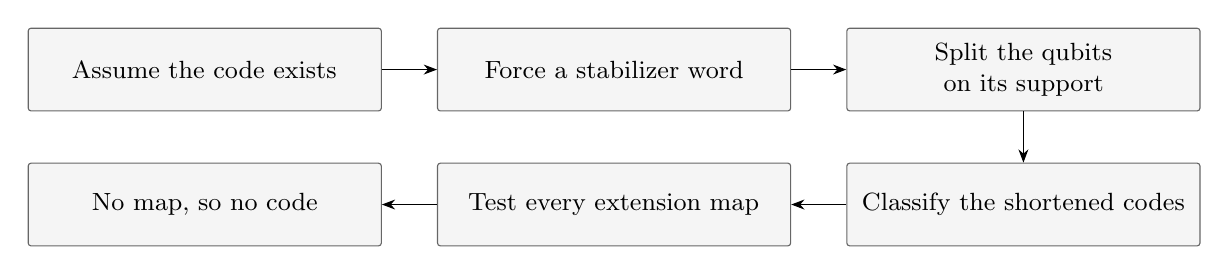
\begin{tikzpicture}[>=Stealth,
 proofbox/.style={draw=black!60,fill=black!4,rounded corners=1pt,
 text width=4.25cm,minimum height=1.05cm,align=center,font=\small},
 node distance=0.65cm and 0.7cm]
\node[proofbox] (assume) {Assume the code exists};
\node[proofbox,right=of assume] (force) {Force a stabilizer word};
\node[proofbox,right=of force] (split) {Split the qubits on its support};
\node[proofbox,below=of split] (classify) {Classify the shortened codes};
\node[proofbox,left=of classify] (test) {Test every extension map};
\node[proofbox,left=of test] (none) {No map, so no code};
\draw[->] (assume)--(force);
\draw[->] (force)--(split);
\draw[->] (split)--(classify);
\draw[->] (classify)--(test);
\draw[->] (test)--(none);
\end{tikzpicture}
\caption{The structural reduction and the finite extension test.}
\label{fig:proof-flow}
\end{figure}

A first reading can follow the definitions in Section~\ref{sec:extension}
and the fourteen-qubit example in Section~\ref{sec:fourteen}, where the
counting inequality finishes the proof. Sections~\ref{sec:sixteen} and
\ref{sec:seventeen} apply the same setup to the two main targets;
Section~\ref{sec:computation} explains why their finite lists are complete.

\subsection{The extension criterion}

A coset of a subspace consists of all vectors obtained by adding its
members to one fixed vector. The quotient is the vector space of these
cosets: it treats two vectors as equivalent when their difference lies
in that subspace. Here this identifies local Pauli words that differ by
a stabilizer supported on the selected coordinates.

Put \(E=R_T^\perp/R\). Write \(c_R(e)\) for the minimum weight of a
representative of \(e\in E\), and write \(\delta(u)\) for the minimum
weight of a coset \(u\) of \(C\). In suitable coordinates, an extension
is described by a binary matrix \(M\) satisfying
\begin{equation}\label{eq:intro-criterion}
 \Gamma=MJM^\tr,\qquad c_R(e)+\delta(Me)\geq d\quad(e\ne0).
\end{equation}
Here \(J\) is the symplectic matrix on \(E\), and \(\Gamma\) is the
Gram matrix of a basis of \(C^\perp\). The first equation is the
commutation condition. The second states that the least weight in each
corresponding pair of cosets is at least \(d\).

Theorem~\ref{thm:extension} proves that these conditions are necessary
and sufficient when \(d(C)\geq d\) and every stabilizer word of weight
below \(d\) lies in \(R\). This includes pure codes and codes whose
degeneracy is confined to the selected coordinates.
Theorem~\ref{thm:relative} gives a relative-distance version without
this restriction. In that version, the relevant coset minima also depend
on \(M\).

For example, suppose \(R=\langle ZZZZ\rangle\) on four coordinates.
Here \(I\) denotes the identity and \(Z\) a nonidentity Pauli letter.
The local class \(ZIII+R=\{ZIII,IZZZ\}\) has minimum weight one.
If its image under \(M\) had coset minimum weight three, the two
parts could be combined into a centralizer word of weight four outside
\(R\). In the setting of Theorem~\ref{thm:extension}, this rules out
distance five. The inequality in \eqref{eq:intro-criterion} makes this
test for every local class at once.

Every nonzero element of \(\ker M\) represents a logical operator
supported entirely on \(T\). The weights and symplectic products of these operators restrict the hull
\(C\cap C^\perp\) of the shortened code. A further counting condition
compares cosets of \(C\) of small weight with classes in \(E/\ker M\)
of sufficiently large weight. These restrictions can exclude a shortened
code before its extension matrices are enumerated.

\subsection{Applications: the two nonexistence proofs}

For sixteen qubits, exact weight-enumerator certificates and an integer
congruence show that a hypothetical code is pure and has minimum
stabilizer weight \(m\in\{6,7,8,9\}\). Shortening the centralizer on
the support of such a word gives one of four additive-code classifications,
containing 3,957 equivalence classes altogether. None admits a map
satisfying the distance inequalities in \eqref{eq:intro-criterion}.
The commutation equation is not needed in this case: even this relaxation
has no solution.

For seventeen qubits, purity alone leaves a less convenient collection
of shortening cases. We instead prove that every hypothetical code has
a stabilizer word of weight eight. A quadratic-form argument bounds the
binary dimension of the shortened nine-coordinate code by six. It follows
that there are just five possible local stabilizers \(R\): one of rank
one and four of rank two. The rank-one type has five admissible kernel cases,
determined by the kernel dimension, restricted symplectic rank, and
shortened-code hull.
These restrictions reduce the remaining problem to complete classifications
on nine coordinates and finite extension searches.

As a smaller application, Section~\ref{sec:fourteen} gives the
fourteen-qubit argument in the same notation. There a unique weight-four
stabilizer word forces \(\ker M=0\). Of the 37 possible shortened
codes, 25 have the wrong hull dimension and the remaining 12 violate the
coset-counting condition. The final contradiction requires no search over
extension matrices.

\subsection{Previous work}

The symplectic representation of stabilizer codes and the MacWilliams and
shadow identities are standard \cite{crss,rains}. Gundersen et al.
\cite{puncturing} describe puncturing directly in symplectic and stabilizer
matrix notation. Complementary symplectic projections are treated in
\cite{anticodes}; related subspace constructions appear in the use of
Goursat's lemma for subsystem codes \cite{goursat} and in
entanglement-assisted error correction \cite{catalytic}.
Our extension criterion uses this linear algebra while retaining the
minimum weights in the original coordinate blocks. Its role here is to
derive the kernel and coset-counting restrictions and to specify the
finite problems used in the two nonexistence proofs.

Classification by extension and the use of automorphism groups are also
established methods \cite{kaski}. We use the distance-five additive-code
classifications of Grassl et al. \cite{dodeca}, and give completeness
checks for the additional classifications needed here. Earlier quantum
nonexistence proofs combining structural reductions and finite searches
include the \(\qc{13,5,4}\) result of Bierbrauer et al. \cite{bierbrauer}.
Related geometric methods for purity and local structure are developed
in \cite{geometry}.

The semidefinite-programming bounds with rational certificates in \cite{sdp}, Table~1,
leave code-space dimension \(K=32\) possible at \((n,d)=(16,5)\),
and \(K=8\) possible at \((17,6)\): their displayed intervals are
\(32\leq K\leq42\) and \(4\leq K\leq8\), respectively.
Theorem~\ref{thm:main} excludes the corresponding stabilizer codes by
using their additional algebraic structure.

Singh \cite{singh} announced the \(\qc{14,3,5}\) nonexistence result,
including degenerate codes, on 10 August 2026. Section~\ref{sec:fourteen}
gives a hull-and-coset argument as a worked application of the extension
criterion.

Lai \cite{lai} develops refined weight-enumerator and structural tests.
His Table~II records the intermediate candidate counts; Section~VII-D
leaves 27 candidate distributions for \(\qc{16,5,5}\) and seven for
\(\qc{17,3,6}\), with nonexistence unestablished for either parameter
set. The present proofs exclude both parameter sets through complete
shortened-code classifications and extension tests.

The computational premises, verification coverage, and data limits are
described in Section~\ref{sec:computation} and
Appendix~\ref{app:evidence}.

\subsection{Organization}

Section~\ref{sec:extension} proves the extension criterion.
Section~\ref{sec:obstructions} derives the kernel, hull, and coset-counting
bounds, including a redundancy bound when the local stabilizer is a
full-support plane. Sections~\ref{sec:fourteen}, \ref{sec:sixteen}, and
\ref{sec:seventeen} give the applications in increasing computational complexity. Section~\ref{sec:computation} describes classification
completeness and the computational verification. The appendices specify
the exact certificates, the extension algorithms, and the available data.

\section{An extension criterion for stabilizer codes}\label{sec:extension}

\subsection{Pauli space, distance, and degeneracy}

All vector spaces are over \(\F\). Write
\[
 V_n=\F^{2n}=\{(x\mid z):x,z\in\F^n\},\qquad
 \langle(x\mid z),(x'\mid z')\rangle=x\cdot z'+z\cdot x'.
\]
At each coordinate, the pairs \((0,0),(1,0),(0,1),(1,1)\) represent
\(I,X,Z,Y\), respectively, with scalar phases omitted. Vector addition
then represents multiplication of Pauli operators up to phase. The
symplectic product is zero for commuting operators and one for
anticommuting operators. The support of a word is the set of coordinates
where its letter is not \(I\).
The Pauli weight is \(\wt(x\mid z)=|\{i:(x_i,z_i)\ne(0,0)\}|\).
A \(Z\)-only word has letters \(I\) and \(Z\), so its \(X\)-component vanishes.
A stabilizer is represented by its binary subspace; Pauli phases are omitted.
A subspace is isotropic if every pair of its words has symplectic product zero.
A binary \(\qc{n,k}\) stabilizer is an isotropic subspace
\(S\leq V_n\) of dimension \(n-k\). Its centralizer is \(D=S^\perp\),
of dimension \(n+k\). For a Pauli stabilizer this commuting space is
also called its normalizer. For \(k>0\) its distance is
\[
 d(S)=\min\{\wt(w):w\in S^\perp\setminus S\}.
\]
The encoded states are the common eigenspace of independent commuting
generators. The centralizer contains the Pauli operators commuting with
all these generators; its elements outside \(S\) act nontrivially on
the encoded information. Stabilizer words themselves act trivially there,
so a low-weight stabilizer word is permitted. A code is pure to distance
\(d\) when every nonzero word of its centralizer has weight at least \(d\).
For a code of distance at least \(d\), degeneracy at that threshold
means that \(S\) contains a nonzero word of weight below \(d\).
An additive code here is an \(\F\)-linear subspace of Pauli space;
it need not be isotropic. For an additive code \(C\), \(d(C)\) means the
minimum weight of a nonzero codeword, with \(d(\{0\})=+\infty\).
The notation \((\ell,2^c,d)_4\) means an additive code of length
\(\ell\), binary dimension \(c\), and minimum distance \(d\) over
the four-letter Pauli alphabet.

Write \(A_j\) for the number of stabilizer words of weight \(j\); their
list is the weight enumerator. Two additive codes are physically equivalent
if a permutation of coordinates and independent permutations of
\(X,Y,Z\) at each coordinate carry one onto the other. These relabelings
preserve weight and commutation.

Split the coordinates into \(T\), of size \(m\), and its complement,
of size \(f=n-m\). Write \(V_n=V_T\oplus W\), with \(W=V_f\).
We view \(V_T\) and \(W\) as subspaces of \(V_n\) by padding with
identity letters on the other coordinates. Write \(\pi_T\) and
\(\pi_W\) for the two coordinate projections. A prefix is a word on
\(T\), and a suffix is a word on its complement.

\begin{center}\small
\begin{tabularx}{\linewidth}{@{}lX@{}}\toprule
Symbol&Meaning\\\midrule
\(n,k,d\)&Physical qubits, encoded qubits, and target distance\\
\(S,D=S^\perp,A_j\)&Stabilizer, centralizer, and stabilizer weight counts\\
\(T,m,f\)&Selected support, its size, and complementary size \(n-m\)\\
\(R,r\)&Stabilizer supported on \(T\), and its dimension\\
\(C,P=C^\perp\)&Shortened centralizer, and its dual on the complement\\
\(E,a,b\)&Local quotient \(R_T^\perp/R\), its dimension, and \(\dim P\)\\
\(M,\tau,\Gamma\)&Extension map, its symplectic adjoint, and the Gram matrix on \(P\)\\
\(K,q,t\)&Kernel of \(M\), its dimension, and its restricted form rank\\
\(N,h\)&Kernel of \(\tau\), and hull dimension \(\dim(C\cap C^\perp)\)\\
\(H,Q\)&Local centralizer \(S^\perp\cap V_T\), and syndrome image \(\im M\)\\
\(\sigma,c_R,\delta\)&Syndrome map, local coset minimum weight, and complementary coset minimum weight\\
\(\varepsilon,\mathcal{K}_j^\ell\)&Weight-parity function and quaternary Krawtchouk polynomial\\
\(\mu\)&Half the local quotient dimension in the search appendix\\\bottomrule
\end{tabularx}
\end{center}

\subsection{The local quotient and the shortened code}

The local data have different roles. The space \(R=S\cap V_T\)
records stabilizer words supported on \(T\); the shortened centralizer
\(C=S^\perp\cap W\) records centralizer words supported on its
complement. We now prescribe \(R\) and \(C\) and ask which full
stabilizers can have these two spaces.
Fix an isotropic subspace \(R\leq V_T\) of dimension \(r\), where
\(0\leq r\leq m\), and define
\[
 E=R_T^\perp/R,\qquad a=\dim E=2m-2r.
\]
Here \(R_T^\perp\) is the orthogonal complement of \(R\) within
\(V_T\).
An element of \(E\) is a coset \(v+R\): two local operators are
identified when their difference is a local stabilizer. This identification
retains their possible logical action, while the function below retains
their least physical weight.
The quotient carries a nondegenerate symplectic form. Fix a symplectic basis with matrix
\(J=\left[\begin{smallmatrix}0&I\\I&0\end{smallmatrix}\right]\).
For \(e\in E\), define
\[
 \cost(e)=\min_{v+R=e}\wt(v).
\]
\(c_R\) is the minimum coset weight in the original coordinate block.
An arbitrary
symplectic change of basis need not preserve it.

The dimension required of \(C\) follows from projection and rank--nullity.
For an actual extension, a vector on \(T\) is orthogonal to
\(\pi_T S^\perp\) if and only if it lies in \(S\cap V_T=R\).
\(\pi_T S^\perp=R_T^\perp\), of dimension \(2m-r\).
Its projection kernel is \(C\), so
\(\dim C=(n+k)-(2m-r)\).
Fix an additive code \(C\leq W\) of binary dimension
\(n+k-2m+r\), assumed to lie between zero and \(2f\). Put
\[
 P=C^\perp_W,\qquad b=\dim P=n-k-r.
\]
Orthogonal complements of \(C\) and \(P\) are taken inside \(W\).
Choose a basis \(v_1,\ldots,v_b\) of \(P\), set
\(\Gamma_{ij}=\langle v_i,v_j\rangle\), and identify \(W/C\)
with \(\F^b\) by the surjective syndrome map
\[
 \sigma(w)_j=\langle v_j,w\rangle,\qquad
 \delta(u)=\min\{\wt(w):\sigma(w)=u\}.
\]
Its kernel is \(C\). In particular \(\delta(0)=0\), regardless of
\(d(C)\). A syndrome \(u\) is a label for one coset of
\(C\), and \(\delta(u)\) is the smallest weight of any word with
that label.

For a subspace \(U\), its radical is
\(\rad(U)=\{u\in U:\langle u,v\rangle=0\text{ for every }v\in U\}\).
For a code, this same intersection with its dual is called its hull.
The nullspace of \(\Gamma\) represents \(\rad(P)=P\cap P^\perp
=C^\perp\cap C\). The binary nullity of \(\Gamma\) is
\(h=\dim(C\cap C^\perp)=\dim\Hull(C)\).

For reference, the four spaces used in the extension criterion are:
\begin{center}\small
\begin{tabularx}{\linewidth}{@{}lXl@{}}\toprule
Space&Meaning&Binary dimension\\\midrule
\(R\)&Stabilizer words supported on \(T\)&\(r\)\\
\(E\)&Local operators commuting with \(R\), modulo \(R\)&\(a=2m-2r\)\\
\(C\)&Centralizer shortened on \(T\)&\(n+k-2m+r\)\\
\(P=C^\perp\)&Projections of stabilizer words onto the complement&\(b=n-k-r\)\\\bottomrule
\end{tabularx}
\end{center}

\subsection{Reconstructing the full stabilizer}

The matrix \(M\) specifies which suffix coset accompanies each local
class. Its entries alone do not guarantee a code: the two coordinate
blocks must give commuting stabilizer words, and their combined weights
must satisfy the distance requirement. These are the two conditions in
the following theorem.

\begin{theorem}[Stabilizer extension criterion]\label{thm:extension}
Assume \(0<k<n\) and \(d(C)\geq d\), with \(R,C\) and their dimensions
as above.
There is a bijection between:
\begin{enumerate}[label=(\roman*)]
\item isotropic stabilizers \(S\) of dimension \(n-k\) satisfying
\[
 S\cap V_T=R,\quad S^\perp\cap W=C,\quad
 \wt(v)\geq d\ \text{for every }v\in S^\perp\setminus R;
\]
\item matrices \(M\in\F^{b\times a}\) satisfying
\begin{equation}\label{eq:exact}
 \Gamma=MJM^\tr,\qquad
 \cost(e)+\delta(Me)\geq d\quad(0\ne e\in E).
\end{equation}
\end{enumerate}
The stabilizer corresponding to \(M\) is \(S_M=D_M^\perp\), where
\begin{equation}\label{eq:graph-D}
 D_M=\{(v,w):v\in R_T^\perp,\ \sigma(w)=M(v+R)\}.
\end{equation}
The weight hypothesis in (i) is equivalent to distance at least \(d\)
together with localization of every stabilizer word of weight below \(d\)
inside \(R\).
\end{theorem}

\begin{proof}
\emph{Recovering the attachment map.}
Let \(S\) satisfy (i), and put \(D=S^\perp\). The annihilator of
\(\pi_TD\) inside \(V_T\) is \(S\cap V_T=R\); hence
\(\pi_TD=R_T^\perp\). The kernel of \(\pi_T|_D\) is \(C\).
For each \(v\in R_T^\perp\), the corresponding words on the
complement of \(T\) form a nonempty coset of \(C\). Addition in \(D\) makes this coset assignment linear. Since \(R\subseteq S\subseteq D\), it depends only
on \(e=v+R\), defining \(M:E\to W/C\).

For \(e\ne0\), its prefix representatives and the members of its suffix
coset can be chosen independently, by adding \(R\) and \(C\).
Their minimum total weight is
\(\cost(e)+\delta(Me)\). All lie outside \(R\), proving the inequality.
The suffix-only fiber gives \(d(C)\geq d\).

\emph{Recovering the commutation condition.}
The duality between projection and shortening also gives \(\pi_WS=P\). Indeed,
a word on \(W\) annihilates \(\pi_WS\) if and only if its extension
by zeros belongs to \(S^\perp\cap W=C\), so
\((\pi_WS)^\perp_W=C\). The kernel of
\(\pi_W|_S\) is \(R\), so \(S/R\) is the graph of a linear map
\(\tau:P\to E\). Write \(A\) for its \(a\)-by-\(b\) coordinate matrix.
For \(x=\sum c_jv_j\), this graph has prefix class \(Ac\).
Commutation with a centralizer word of prefix class \(e\) gives
\(e^\tr JAc+c^\tr Me=0\) for every \(e,c\). Thus
\(M=A^\tr J\), equivalently \(A=JM^\tr\). Two graph words
commute if and only if their local and complementary symplectic products
cancel. Isotropy of the graph gives
\(\Gamma=A^\tr JA=MJM^\tr\). \(\tau\) is the symplectic
adjoint of \(M\).
Its kernel has a direct interpretation: \(\tau(x)=0\) means that
a stabilizer projecting to \(x\) has local part in \(R\), which can
be removed by adding that local stabilizer. \(\ker\tau=S\cap W\).

\emph{Constructing a stabilizer from the map.}
Conversely, let \(M\) satisfy (ii) and define \(D_M\) by
\eqref{eq:graph-D}. Its projection is \(R_T^\perp\), its suffix-only
kernel is \(C\), and it contains \(R\). Consequently
\(\dim D_M=2m-r+\dim C=n+k\), so \(\dim S_M=n-k\),
and annihilator duality gives \(S_M\cap V_T=R\).
For a projected stabilizer word \(x=\sum c_jv_j\), commutation with
\(D_M\) forces its prefix class to be \(JM^\tr c\). The symplectic product of
two such words is
\(c^\tr(MJM^\tr+\Gamma)c'=0\). The local words of \(R\) commute
with them because their prefixes lie in \(R_T^\perp\). \(S_M\)
is isotropic.

Every fiber of nonzero prefix class has weight at least \(d\) by (ii).
In the zero-class fiber, the prefix lies in \(R\) and the suffix lies in
\(C\); a word outside \(R\) has a nonzero suffix, of weight at least
\(d\). This proves (i). The fibers determine \(D\) and therefore
\(S=D^\perp\) uniquely, establishing the bijection.
\end{proof}

\subsection{A relaxation using only coset weights}

The distance inequalities do not generally imply commutation. For example,
take \(n=4,k=1,d=2\), \(R=\langle ZZ\rangle\), and
\(C=\langle XX,ZZ\rangle\) on the other two sites. In the prefix basis
\(Z_0,X_0X_1\), the nonzero coset minimum weights are \(1,2,2\). Choose independent
nonzero syndrome columns. All weight inequalities hold, since the three
nonzero cosets of \(C\) have distance one. But \(C\) is self-dual,
so \(\Gamma=0\), whereas \(MJM^\tr\ne0\).
Excluding all weight-admissible maps still excludes genuine extensions.
Finding one such map would not construct a code.

\subsection{Extensions of degenerate codes}

For an arbitrary degenerate code, \(C\) may contain short stabilizer words.
The same graph construction still applies, with the distance taken relative
to the reconstructed stabilizer.

\begin{theorem}[Relative extension criterion]\label{thm:relative}
Keep \(R,C,E,P\) and their dimensions, but impose no lower bound on
\(d(C)\). Let \(M\) satisfy \(\Gamma=MJM^\tr\), and define
\(\tau_M(\sum c_jv_j)=JM^\tr c\), and
\[
 \delta_M^{\rm log}(e)=\min\{\wt(w):\sigma(w)=Me,\
             w\notin\tau_M^{-1}(e)\},
\]
where \(\tau_M^{-1}(e)\) is a subset of \(P\), and the minimum of
the empty set is \(+\infty\).
Then \(S_M\) has distance at least \(d\) if and only if
\[
 \cost(e)+\delta_M^{\rm log}(e)\geq d\quad\text{for every }e\in E,
\]
including \(e=0\).
\end{theorem}
\begin{proof}
The graph and dimension arguments above do not require a distance assumption.
A word \((v,w)\in D_M\), with \(v+R=e\), is in \(S_M\) if and only if
\(w\in P\) and \(\tau_M(w)=e\). Membership is independent of the
representative of \(e\), because \(R\subseteq S_M\). The displayed
minimum ranges over precisely the suffixes of logical words in
that fiber. Prefix and suffix representatives vary independently. Minimizing
their sum gives the assertion, fiber by fiber.
\end{proof}

At \(e=0\), the suffix minimum is the distance of \(C\) relative to
\(N=\ker\tau_M\): it is \(\min\{\wt(w):w\in C\setminus N\}\).
The coset minimum depends on \(M\), so the theorem does not supply a fixed
precomputed table of coset minimum weights for arbitrary degeneracy. The searches below
use Theorem~\ref{thm:extension} only after proving purity or localization.

\section{Restrictions on extension kernels}\label{sec:obstructions}

We derive necessary conditions from the kernel and image of the extension
map. Throughout this section, \(S\) is a stabilizer with
\(S\cap V_T=R\), \(S^\perp\cap W=C\), and extension map \(M\).
Every nonzero kernel element represents a logical operator supported on
\(T\).
There are two kernels to distinguish. The kernel \(K=\ker M\) records
logical operators supported on \(T\). The kernel \(N=\ker\tau\)
records stabilizer words supported on the complementary coordinates:
their projected local class is zero, and an element of \(R\) removes
the remaining local representative. The hull identities below relate
these two kinds of local information.

\begin{proposition}[Kernel and hull identities]\label{prop:kernel}
For an extension, put \(K=\ker M\), \(q=\dim K\), and let \(t\) be the
rank of the symplectic form restricted to \(K\). Then
\begin{align}
 \rank\Gamma&=a-2q+t,&
 h&=b-a+2q-t,\label{eq:hull}\\
 N:=\ker\tau&\subseteq\rad(P),&
 \dim N&=b-a+q.\label{eq:N}
\end{align}
Every nonzero \(e\in K\) has \(\cost(e)\geq d(S)\), even without
purity. Moreover \(q-t/2\leq k\).
\end{proposition}
\begin{proof}
The adjoint map has image \(K^\perp_E\), of dimension \(a-q\).
To see this directly, \(e\) annihilates \(\im\tau\) if and only
if \(\langle e,\tau(x)\rangle=0\) for every \(x\in P\), or
equivalently \(Me=0\). Nondegeneracy of \(E\) then gives
\(\im\tau=K^\perp_E\).
The radical of its restricted form is \(K\cap K^\perp\), of dimension
\(q-t\) by rank--nullity on the restricted form. Pullback along the surjection \(P\to K^\perp\) leaves
the form rank unchanged, giving \(a-q-(q-t)\). Subtracting from \(b\)
gives \eqref{eq:hull}. The map \(\tau\) has rank \(a-q\), giving
\eqref{eq:N}; a vector in its kernel pairs trivially with all of \(P\).

For \(e\ne0\) in \(K\), a prefix representative with zero suffix lies
in \(S^\perp\). It cannot lie in \(S\), because \(S\cap V_T=R\).
Its minimum weight is at least the logical distance. The space
\(K\) embeds in the \(2k\)-dimensional nondegenerate logical space
\(S^\perp/S\). A subspace of dimension \(q\) and form rank \(t\)
has an isotropic subspace of dimension \(q-t/2\); that dimension is at
most \(k\).
\end{proof}

\subsection{Counting cosets of small weight}

Let \(Q=\im M\). The syndrome subspace \(Q\) is naturally
\(N^\perp_W/C\): these are precisely the suffix classes annihilating
\(N=\ker\tau\). The map \(M\) induces a bijection \(E/K\to Q\).
For \(\eta\in E/K\), put
\(\kappa(\eta)=\min_{e\in\eta}\cost(e)\).
\(\kappa(\eta)\) is the least weight available among all local
classes that have the same suffix image. If that suffix image has small
minimum weight, every one of its possible local partners must compensate
with a sufficiently large weight. Counting these partners gives the next
inequality.

\begin{proposition}[Coset-counting inequality]\label{prop:capacity}
In the localized setting of Theorem~\ref{thm:extension}, for
\(0\leq j<d\),
\begin{equation}\label{eq:capacity}
 |\{0\ne u\in Q:\delta(u)\leq j\}|
 \leq |\{0\ne\eta\in E/K:\kappa(\eta)\geq d-j\}|.
\end{equation}
If every nonzero class in \(E\) has minimum weight below \(d\), then
\[
 K=0,\quad h=b-a,\quad N=\rad(P),\quad Q=\im\Gamma.
\]
\end{proposition}
\begin{proof}
For a fixed \(\eta\), all its members have the same syndrome image.
Minimizing \eqref{eq:exact} over them gives
\(\kappa(\eta)+\delta(M\eta)\geq d\).
Each nonzero syndrome class of minimum weight at most \(j\) therefore
corresponds to a distinct nonzero coset in \(E/K\) whose minimum weight
is at least \(d-j\). This proves the inequality.
The minimum-weight hypothesis and Proposition~\ref{prop:kernel} imply
\(K=0\). Then \eqref{eq:hull} and \eqref{eq:N} give the remaining
statements, with \(\im\Gamma=(\ker\Gamma)^\perp\) in syndrome
coordinates.
\end{proof}

Violation of \eqref{eq:capacity} excludes an extension without enumerating
the matrices \(M\). The inequality alone is not sufficient for existence.

\subsection{A binary bound for a rank-one local stabilizer}

\begin{proposition}[Kernel projection bound]\label{prop:griesmer}
Suppose \(R=\langle Z^m\rangle\) and \(d>\lfloor m/2\rfloor\).
The physical \(X\)-projection maps \(K\) injectively to an even binary
linear code of length \(m\), dimension \(q\), and distance at least
\(\Delta=2(d-\lfloor m/2\rfloor)\). Consequently,
\begin{equation}\label{eq:griesmer}
 m\geq\sum_{i=0}^{q-1}\left\lceil\frac{\Delta}{2^i}\right\rceil.
\end{equation}
\end{proposition}
\begin{proof}
Adding \(Z^m\) leaves the \(X\)-mask unchanged, so this projection is
well defined on \(E\). Commutation with \(Z^m\) makes its weight
\(w\) even. If \(z\) counts \(Z\)-letters off that mask, then
\[
 \cost(e)=w+\min(z,m-w-z)\leq\lfloor m/2\rfloor+w/2.
\]
A nonzero class represented by a \(Z\)-only word has minimum weight at most \(\lfloor m/2\rfloor\),
so cannot lie in \(K\). This proves injectivity, and
\(\cost(e)\geq d\) gives \(w\geq\Delta\).
The last inequality is the binary Griesmer bound applied to that projected
code. For completeness, choose a minimum-weight binary word of weight
\(w\). Puncturing its support leaves a code of dimension one less and
distance at least \(\lceil w/2\rceil\): the two representatives of a
nontrivial quotient class have weight sum equal to \(w\) plus twice
their common suffix weight, and each has weight at least \(w\).
Only zero and the chosen word can lie wholly in that support. Induction
gives the stated sum.
\end{proof}

The binary Griesmer bound applies to the projected kernel. For \(m=8,d=6\), it gives \(q\leq4\).
Section~\ref{sec:seventeen} sharpens this to three using parity and the
logical symplectic dimension.

\subsection{Balanced local planes and redundancy}

When the local stabilizer is generated by two full-support words, the
minimum-weight condition determines the symbol counts of every nonzero
kernel class. This gives the following restriction.

\begin{theorem}[Balanced-plane obstruction]\label{thm:balanced}
Suppose \(S\cap V_T=R=\langle X^m,Z^m\rangle\), where \(m=4\omega\),
\(\omega\geq1\), and \(d(S)\geq3\omega\). Then \(2^q\leq m\).
If \(\omega\) is even, \(K\) is isotropic. If \(\omega\) is odd, then
\(q\leq2\), with restricted form rank zero for \(q\leq1\) and two
for \(q=2\). In particular,
\[
 \begin{array}{ll}
 n-k\geq2m-2-\lfloor\log_2m\rfloor,&\omega\text{ even},\\
 n-k\geq2m-4,&\omega\text{ odd}.
 \end{array}
\]
No purity assumption is needed.
\end{theorem}
\begin{proof}
For a word on \(T\), let \(n_I,n_X,n_Y,n_Z\) be its four symbol
counts. Addition of \(R\) permutes the four counts, so the minimum
weight modulo \(R\) is \(m-\max n_L\leq3m/4\). A nonzero kernel class has minimum weight
at least \(3\omega\); hence every count is \(\omega\). All four words in that
class have weight \(3\omega\).

Let \(\widetilde{K}\) be the preimage of \(K\) in \(R_T^\perp\), and put
\(L=|\widetilde{K}|=2^{q+2}\). Its weight enumerator is
\(1+(L-4)z^{3m/4}+3z^m\). The second MacWilliams coefficient of its
dual equals
\[
 \frac{6m^2}{L}-\frac{3m}{2}.
\]
This coefficient counts weight-two words in the dual code. It is
nonnegative, so \(L\leq4m\), or \(2^q\leq m\).

The Pauli parity function \(\varepsilon(v)=\wt(v)\bmod2\) satisfies
\begin{equation}\label{eq:polar}
 \varepsilon(u+v)=\varepsilon(u)+\varepsilon(v)+\langle u,v\rangle.
\end{equation}
If \(\omega\) is even, all words of \(\widetilde{K}\) are even, so \(\widetilde{K}\), and hence
\(K\), is isotropic. If \(\omega\) is odd, two distinct nonzero kernel
classes pair to one, since the three representatives involved have odd
weight. Three independent classes would contradict bilinearity:
\(\langle u,v+w\rangle=1+1=0\), although the same rule requires one.
\(q\leq2\), with the asserted ranks.

Here \(a=2m-4\), \(b=n-k-2\). In the even case,
\(\rank M=a-q\leq b\) gives \(n-k\geq2m-2-q\).
In the odd case, the smallest possible \(\rank\Gamma=a-2q+t\)
is \(a-2\), so \(b\geq a-2\), giving the second bound.
\end{proof}

For example, the specified local plane on twelve coordinates at distance
at least nine requires \(n-k\geq20\). The hypothesis fixes the entire stabilizer supported on those twelve
coordinates; the conclusion applies to codes with that local structure.

\subsection{Choosing a tractable support}

\begin{proposition}[Support selection]\label{prop:support}
Let \(B(f,d)\) be an upper bound on the binary dimension of an additive
length-\(f\), minimum-distance-\(d\) code. If the stabilizer of a pure
\(\qc{n,k,d}\) code contains a nonzero word with support \(T\),
where \(|T|=m\), then \(r=\dim(S\cap V_T)\) satisfies
\[
 1\leq r\leq B(n-m,d)-n-k+2m.
\]
\end{proposition}
\begin{proof}
The shortened centralizer has dimension \(n+k-2m+r\) by
Theorem~\ref{thm:extension}'s projection argument, and distance at least
\(d\) by purity. Apply the additive dimension bound.
\end{proof}

The selected word need not have minimum stabilizer weight. This freedom
is useful when an exact enumerator certificate forces a particular weight
whose complement is already classifiable.

\section{A supporting application: fourteen qubits}\label{sec:fourteen}

We apply the kernel and coset-counting conditions to fourteen qubits.
The existence question is Research Problem 1 of Ball, Centelles, and Huber
\cite{ball}.
The parameter conclusion was previously announced by Singh
\cite{singh}. We give a hull-and-coset proof as an application of the
extension criterion. This example shows that the kernel conditions can exclude extensions
without enumerating their matrices, even when the code is degenerate.

\begin{proposition}[Fourteen-qubit local reduction]\label{prop:14-local}
A hypothetical \(\qc{14,3,d\geq5}\) code has exactly one nonzero
stabilizer word of weight at most four. That word has weight four.
\end{proposition}
\begin{proof}
The ordinary enumerator/shadow identity in the repository gives
\[
 11685888A_1+1345536A_2+4681728A_3+989184A_4\leq3336192.
\]
Integrality implies \(A_1=A_3=0\), \(A_2\leq2\), \(A_4\leq3\).
A further exact congruence gives \(A_3+A_4\equiv1\pmod2\), hence
\(A_4\in\{1,3\}\). It is obtained from the total row, low-weight
MacWilliams rows, and signed shadow equalities with multipliers
\[
 (1,-2,-6,-17,-95;\ -20,-24,1108,246)
\]
in the order total; low rows one through four; shadow equalities zero
through three. Modulo 4096 only the coefficients of \(A_3,A_4\)
survive, both equal to 2048, and the right-hand side is 2048.

An exact split-coset certificate excludes a weight-two stabilizer word.
For distinct commuting weight-four words, let \(\iota\) be their support
intersection size and \(u\) the number of different letters on that
intersection. Then \(u\) is even and their sum has weight \(8-2\iota+u\).
All cases with \(\iota\geq2\) are excluded as follows:
\begin{center}\small
\begin{tabular}{@{}ccl@{}}\toprule
\(\iota\)&\(u\)&Obstruction\\\midrule
4&2&Their sum has weight two.\\
4&4&Certificate for \(\langle XXXX,ZZZZ\rangle\).\\
3&0&Their sum has weight two.\\
3&2&Certificate for \(\langle XXZZI,ZZZIZ\rangle\).\\
2&0&Certificate for \(\langle ZZZZII,ZZIIZZ\rangle\).\\
2&2&Certificate for \(\langle ZZZZII,XXIIXX\rangle\).\\\bottomrule
\end{tabular}
\end{center}
If \(\iota=4,u=0\), the words are identical. Distinct weight-four
words intersect in at most one site, with equal letters there. All such
words may be made \(Z\)-only by one consistent local Clifford map.

If \(A_4=3\), the three words are independent: the sum of two has weight
six or eight, never four. Their three supports have pairwise intersection
sizes zero or one. The intersection graph has zero, one, two, or three
edges; when it has three, either the intersections are distinct or there
is one common site. These give exactly five support geometries. Their
union sizes are 12, 11, 10, 9, and 10, respectively. Exact rank-three
coset certificates exclude each geometry, with the disjoint one using
three four-site blocks and a two-site suffix. All include the already
proved zeros and the assumption \(A_4=3\). The data are in \pathcode{verification/certificates/14/}, with the
standalone checker \pathcode{verification/check_certificates14.py}. \(A_4=1\), proving the assertion.
\end{proof}

Normalize the unique short word to \(p=Z^4\), let \(T\) be its support,
and put \(R=\langle p\rangle\). No other local stabilizer word is
possible, since all words on \(T\) have weight at most four.
The extension theorem applies with localized degeneracy, even though the
code is not pure. Here
\[
 a=6,\quad b=10,\quad C\leq V_{10},\quad\dim C=10,\quad d(C)\geq5.
\]
Every class in \(E\) has minimum weight at most four, forcing \(K=0\). Thus
\(\dim\Hull(C)=b-a=4\) by Proposition~\ref{prop:capacity}.

The minimum weights of the 64 classes in \(E\) have the distribution
\begin{center}
\begin{tabular}{@{}lccccc@{}}\toprule
Minimum weight&0&1&2&3&4\\\midrule
Classes&1&4&27&24&8\\\bottomrule
\end{tabular}
\end{center}
To obtain it directly, group commuting words by their even \(X\)-mask.
The zero mask contributes \(1,4,3\) classes of minimum weight zero, one, and two.
Each of the six weight-two masks contributes four classes of minimum weight two
and four of minimum weight three. The full mask contributes eight classes of
minimum weight four. With \(J_C=\Hull(C)\), the coset-counting inequalities on
\(J_C^\perp/C\) become
\[
 \#\{u\ne0:\delta(u)\leq1\}\leq8,\quad
 \#\{u\ne0:\delta(u)\leq2\}\leq32,\quad
 \#\{u\ne0:\delta(u)\leq3\}\leq59.
\]

There are 37 physical equivalence classes of additive
\((10,2^{10},\geq5)_4\) codes \cite{dodeca}.
Their hull dimensions have multiplicities
\(0:7,\ 2:14,\ 4:12,\ 6:2,\ 8:2\).
25 classes fail the hull requirement. Every one of the remaining
12 violates at least one of the three coset-counting inequalities, as verified
by enumerating physical suffix words and their cosets. No matrix-entry
search is needed at this final step.
This excludes \(\qc{14,3,5}\); the known \(\qc{14,3,4}\)
construction gives \(d_{\max}(14,3)=4\).

The sixteen-qubit \(m=6\) case uses the same 37 ten-coordinate codes,
with a larger local quotient and different coset minimum weights.

\section{The sixteen-qubit exclusion}\label{sec:sixteen}

Assume that \(S\leq V_{16}\) defines a \(\qc{16,5,d\geq5}\) code.
Then \(|S|=2^{11}=2048\). The counts \(A_j\) include products of basis generators.
The argument has three steps. First we prove purity and restrict the
minimum stabilizer weight. Next we show that shortening on such a word
leaves one of four complete code classifications. Finally we test the
extension inequalities on every class in those lists.

\subsection{Purity and minimum stabilizer weight}

\begin{proposition}[Exact low-weight reduction]\label{prop:16-reduction}
Such a code is pure to distance five. Its minimum nonzero stabilizer
weight \(m\) belongs to \(\{6,7,8,9\}\).
\end{proposition}
\begin{proof}
The weight-enumerator equations count words of each weight without
specifying the full code. The MacWilliams identities express centralizer
counts in terms of stabilizer counts, and the shadow identities give
additional nonnegative counts. A certificate is an integer combination
of these necessary relations that gives a contradiction under a stated
case assumption. Its check uses integer arithmetic alone; the general
construction is given in Appendix~\ref{app:certificates}.

The six integer certificates in the repository exclude, in order:
\begin{enumerate}[label=(\alph*)]
\item a stabilizer word of weight one, two, or three;
\item a weight-four stabilizer word together with \(A_4\geq2\);
\item a weight-five stabilizer word under \(A_1=\cdots=A_4=0\);
\item \(A_1=\cdots=A_9=0\).
\end{enumerate}
For a proposed word of weight \(w\), local Clifford operations normalize
it to \(Z^w\). The split system counts complete cosets of
\(\langle Z^w\rangle\), with distance equations through weight four,
centralizer inclusion, and nonnegative shadow coefficients. Every actual
code yields a feasible point. Appendix~\ref{app:certificates} defines
the system and the exact arithmetic checks; the case assumptions and
negative certificate values are tabulated there.

It remains to exclude \(A_4=1\). Write \(\mathcal{K}_j(w)\) for the quaternary
Krawtchouk polynomial at length sixteen, and \(\operatorname{Sh}_j\)
for the shadow counts. Set
\[
 \Delta_0=\sum_wA_w=2048,\quad
 \Delta_j=\sum_w\mathcal{K}_j(w)A_w-2048A_j=0\ (1\leq j\leq4),
\]
and \(\Omega_j=\sum_w(-1)^w\mathcal{K}_j(w)A_w-2048\operatorname{Sh}_j=0\).
In the integer combination
\[
 -740\Delta_0-265\Delta_1-81\Delta_2-19\Delta_3-3\Delta_4
       +80\Omega_0+10\Omega_1-2\Omega_3,
\]
all coefficients vanish modulo \(4096\), except those of
\(A_1,A_2,A_3,A_4\), each congruent to \(2048\).
The right-hand side is \(-740\cdot2048\), which is divisible by
\(4096\).
\(A_1+A_2+A_3+A_4\) is even. The first certificates give
\(A_1=A_2=A_3=0\), \(A_4\leq1\), so \(A_4=0\).
Every centralizer word of weight below five must be a stabilizer;
therefore purity follows. The last two certificate cases give
\(6\leq m\leq9\).
\end{proof}

\subsection{The four shortened-code classifications}

Choose a weight-\(m\) word \(p\) with support \(T\), and normalize
\(p=Z^m\). We first need the \emph{entire} local stabilizer.

\begin{lemma}\label{lem:16-rankone}
For \(m\in\{6,7,8,9\}\), \(S\cap V_T=\langle p\rangle\).
\end{lemma}
\begin{proof}
If \(\dim(S\cap V_T)\geq2\), the shortened centralizer contains a
subcode with parameters
\[
 (10,2^{11},\geq5)_4,\quad(9,2^9,\geq5)_4,
       \quad\text{or}\quad(8,2^7,\geq5)_4
\]
for \(m=6,7,8\), respectively. No additive codes with these parameters exist
\cite{dodeca}; the repository also verifies their emptiness through the
complete lengthening census.
For \(m=9\), an independent local stabilizer word \(\zeta\) and \(\zeta+p\)
must both have weight nine by minimality of \(m\). \(\zeta\) has
\(X\) or \(Y\) at every site of \(T\). It anticommutes with
\(Z^9\) on an odd number of sites, contradicting isotropy.
\end{proof}

The shorter code \(C\) has length \(16-m\), dimension
\(22-2m\), and distance at least five. The quotient \(W/C\) has
dimension ten for every case. The complete classifications contain the following
numbers of physical equivalence classes:
\begin{center}
\begin{tabular}{@{}cccc@{}}\toprule
\(m\)&Shortened length&Binary dimension&Classes\\\midrule
6&10&10&37\\7&9&8&2,298\\8&8&6&1,579\\9&7&4&43\\\bottomrule
\end{tabular}
\end{center}
The four class counts are the exact entries of Table~1 in
Grassl et al. \cite{dodeca}.
The repository reconstructs representatives and checks their completeness
by a second physical graph encoding and orbit--stabilizer mass identities.
The classification procedure is specified in Section~\ref{sec:classification}.

\subsection{The finite prefix-map problem}

For \(R=\langle Z^m\rangle\), use the symplectic basis
\[
 Z_0,\ldots,Z_{m-2},\qquad X_iX_{m-1}\quad(0\leq i<m-1)
\]
of \(E\), with \(Z_{m-1}=\sum_{i<m-1}Z_i\) modulo \(R\).
Each basis image is a ten-bit syndrome. Every actual code gives a linear
map satisfying
\begin{equation}\label{eq:16-weight}
 \cost(e)+\delta(Me)\geq5\qquad(e\ne0).
\end{equation}
Only classes of minimum weight less than five constrain the search.
Omitting \(\Gamma=MJM^\tr\) enlarges the feasible set, so
nonexistence of a map in this larger set is sufficient.

The depth-first traversal assigns basis images and checks each newly
determined subset sum. The forward-checking version maintains every
remaining basis image's allowed domain. A value is removed only when a
specific already determined subset would violate \eqref{eq:16-weight}.
Every word is tested: each \(e\in E\) is a binary sum of the basis
vectors, and its image is the corresponding sum of assigned syndromes.
A Boolean satisfiability (SAT) encoding uses Boolean entries of \(M\), XOR chains
for its values, and a clause for every forbidden element/syndrome pair.
Each forbidden pair is a clause
requiring the entries of \(M\) to avoid that particular map value.
The two encodings construct their coset labels separately.

\begin{lemma}[Physical normalization for the weight-only search]\label{lem:16-symmetry}
If a map satisfying \eqref{eq:16-weight} exists, one exists with
\[
 \xi_0<\xi_1<\cdots<\xi_{m-1},\qquad
 \eta_i<\eta_i+\xi_i\quad(0\leq i<m-1),
\]
where \(\xi_i=M(Z_i)\), \(\eta_i=M(X_iX_{m-1})\), and labels use
any fixed total order.
\end{lemma}
\begin{proof}
The singleton and pair constraints force all \(\xi_i\) to be distinct
and nonzero. A physical permutation of the \(m\) sites fixes \(Z^m\)
and preserves coset minimum weights, so orders the singleton images.
After this permutation, the map is re-expressed in the displayed standard
basis; the dependent image is still
\(\xi_{m-1}=\sum_{i=0}^{m-2}\xi_i\).
The phase operation
\(X\leftrightarrow Y\) on site \(i<m-1\) fixes every \(Z_j\),
fixes the other complementary basis vectors, and replaces
\(X_iX_{m-1}\) by \(X_iX_{m-1}+Z_i\). It exchanges
\(\eta_i\) and \(\eta_i+\xi_i\) independently for each \(i\).
These physical operations preserve all weight inequalities.
\end{proof}

\begin{proposition}[Complete sixteen-qubit extension exclusion]\label{prop:16-search}
None of the 3,957 shortened-code classes admits a map satisfying
\eqref{eq:16-weight}.
\end{proposition}
\begin{proof}[Computer-assisted proof]
The recorded reports cover completed searches for every class.
For \(m\leq8\), a symmetry-free depth-first search and a separately
constructed SAT encoding both exclude every class. For \(m=9\), two
depth-first implementations use Lemma~\ref{lem:16-symmetry}, with
different coset coordinates and search orders. Both exclude all 43 classes.
A known pure \(\qc{16,4,5}\) code is accepted by
both encodings, with and without their symmetry restrictions.
Appendix~\ref{app:search} specifies the finite predicate and completeness
argument; Appendix~\ref{app:evidence} identifies the evidence and its checks.
\end{proof}

Proposition~\ref{prop:16-reduction}, Lemma~\ref{lem:16-rankone}, and
Theorem~\ref{thm:extension} put every hypothetical code into one of these
weight-admissible extension problems. Proposition~\ref{prop:16-search}
excludes them all. This proves the first assertion of
Theorem~\ref{thm:main}.

\section{The seventeen-qubit exclusion}\label{sec:seventeen}

Assume that \(S\leq V_{17}\) is a \(\qc{17,3,d\geq6}\)
stabilizer, so \(\dim S=14\) and \(\dim S^\perp=20\).
The proof first forces a weight-eight stabilizer word. Shortening on its
support leaves nine coordinates, and the dimension bound below permits
one rank-one local stabilizer type and four rank-two types. The rank-one
type then splits into five kernel cases indexed by \((q,t,h)\).
We use \emph{type} for the local stabilizer up to physical equivalence,
\emph{kernel case} for these three invariants, and \emph{weight profile}
for the pair \((A_6,A_7)\). A search part fixes a shortened code, kernels,
and the remaining identification or syndrome data.

\begin{center}\small
\begin{tabularx}{\linewidth}{@{}lXr@{}}\toprule
Local type or kernel case&Exclusion&Shortened-code classes\\\midrule
Rank two: \((6,6,8)\)&Counting leaves 48; extension tests&56\\
Rank two: \((6,8,8)\)&Counting leaves 52; extension tests for each weight profile&56\\
Rank two: \((7,7,8)\)&Counting leaves 52; extension tests&56\\
Rank two: \((8,8,8)\)&Hull restrictions and fixed-kernel extension tests&56\\
Rank one: \((q,t,h)=(1,0,1)\)&Fixed-kernel extension tests&26,752\\
Rank one: \((2,2,1)\)&Fixed-kernel extension tests&26,752\\
Rank one: \((2,0,3)\)&Fixed-kernel extension tests&5,995\\
Rank one: \((3,2,3)\)&Recentering screen and fixed-kernel extension tests&5,995\\
Rank one: \((3,0,5)\)&Recentering screen and binary projection filter&118\\\bottomrule
\end{tabularx}
\end{center}
The repeated class lists in the rank-one rows are tested with different
kernels. The table counts the full input classifications; the proofs
below give the subsequent screens and search counts.

\subsection{A forced support of size eight}

\begin{proposition}[Exact enumerator consequences]\label{prop:17-enumerator}
The hypothetical code is pure to distance six, contains a stabilizer word
of weight eight, and satisfies
\begin{equation}\label{eq:light-budget}
 A_6+A_7\leq2.
\end{equation}
\end{proposition}
\begin{proof}
The split-coset integer certificates for stabilizer weights one through
five exclude all five possibilities without assuming purity. Hence
\(A_1=\cdots=A_5=0\), which implies purity because the logical distance
is at least six. With these zeros imposed, the ordinary enumerator system
plus \(A_8=0\) has an exact infeasibility certificate with negative
right-hand side \(-3,932,160\).

For the last assertion, an integer combination of the ordinary
MacWilliams and shadow relations gives
\(32768(A_6+A_7)\leq65536\). Dividing by 32768 proves
\eqref{eq:light-budget}. Appendix~\ref{app:ordinary17} gives the
multipliers, row definitions, and sign conventions so that the identity
can be checked directly.
\end{proof}

The following additive bound makes the forced support useful. It uses a
parity property that is not visible in the first few nonnegative
MacWilliams coefficients alone.

\begin{lemma}[A nine-coordinate dimension bound]\label{lem:nine-bound}
An additive code on nine sites with minimum distance at least six has
binary dimension at most six.
\end{lemma}
\begin{proof}
A code of larger dimension contains a dimension-seven subcode. Suppose
\(|C|=128\), with nonzero weight counts \(A_6,A_7,A_8,A_9\) summing to
127. The first three nonnegative dual MacWilliams coefficients give
\[
 A_7+2A_8+3A_9\leq102,\qquad
 A_8+3A_9\geq75,\qquad
 3(A_7+A_8)-4A_9\geq17.
\]
The first two imply \(A_7\leq3A_9-48\), hence \(A_9\geq16\), and
also \(A_7+A_8\leq27\). The third then gives \(A_9\leq16\).
Equality forces
\((A_6,A_7,A_8,A_9)=(84,0,27,16)\).

On a binary additive space, weight parity is a quadratic form: its failure
to be additive is the symplectic product in \eqref{eq:polar}.
For a quadratic form \(\varepsilon\) on a \(c\)-dimensional binary space \(U\),
define its Gauss sum by
\[
 G(\varepsilon)=\sum_{v\in U}(-1)^{\varepsilon(v)}.
\]
For weight parity, this is the number of even-weight words minus the
number of odd-weight words. If the polar form has rank \(2\rho\), then
\(G(\varepsilon)\) is zero or \(\pm2^{c-\rho}\). Indeed, squaring the sum and
substituting \(y=x+z\) gives
\[
 G(\varepsilon)^2=2^c\sum_{z\in\rad(U)}(-1)^{\varepsilon(z)}.
\]
The restriction of \(\varepsilon\) to the radical is linear. The last sum is
therefore zero if that restriction is nonzero, and otherwise equals
\(|\rad(U)|=2^{c-2\rho}\). This proves the asserted possibilities.
The forced distribution would instead give Gauss sum
\(128-2\cdot16=96\). Since \(c=7\) and \(0\leq\rho\leq3\),
the possible nonzero absolute values are \(128,64,32,16\), none of
which is 96. This proves the bound.
\end{proof}

Choose a weight-eight stabilizer word \(p\), put \(T=\operatorname{supp}p\),
and normalize \(p=Z^8\). Let \(R=S\cap V_T\), \(r=\dim R\).
The shortened centralizer has length nine and dimension \(4+r\), so
Lemma~\ref{lem:nine-bound} gives \(1\leq r\leq2\).

If \(r=1\), then \(R=\langle Z^8\rangle\).
If \(r=2\), choose \(\zeta\in R\setminus\langle p\rangle\).
Let \(\alpha\) be the number of sites where \(\zeta\) has an \(X\)-component.
It is even by commutation. Since both \(\zeta\) and \(\zeta+p\) have weight
at least six, \(8+\alpha\geq12\), so \(\alpha\in\{4,6,8\}\).
Phase maps fixing \(Z\) remove \(Y\) on those sites. On the other
\(8-\alpha\) sites, let \(\beta\) count the \(Z\)'s of \(\zeta\).
Then \(\alpha+\beta\geq6\) and \(8-\beta\geq6\).
Replacing \(\zeta\) by \(\zeta+p\) exchanges \(\beta\) with \(8-\alpha-\beta\).
Consequently \(\alpha=4\) forces \(\beta=2\); at \(\alpha=6\) we may take
\(\beta=0\) or one; and \(\alpha=8\) forces \(\beta=0\).
Site permutations now give the following list.

\begin{center}
\begin{tabular}{@{}clcc@{}}\toprule
\(\dim R\)&Generators of \(R\)&Nonzero local weights&\(\dim C\)\\\midrule
1&\(Z^8\)&8&5\\
2&\(Z^8,\ XXXXZZII\)&6,6,8&6\\
2&\(Z^8,\ XXXXXXII\)&6,8,8&6\\
2&\(Z^8,\ XXXXXXZI\)&7,7,8&6\\
2&\(Z^8,\ X^8\)&8,8,8&6\\\bottomrule
\end{tabular}
\end{center}

This list covers every possible local stabilizer, with \(R=S\cap V_T\). The shortened-code
classifications contain 32,865 dimension-five classes and 56
dimension-six classes. Section~\ref{sec:computation} gives their completeness arguments.

\subsection{The four rank-two types}

For the types with local weights \((6,6,8)\) and \((7,7,8)\), the local
plane contains two words of weight six or seven. Equality therefore
holds in \eqref{eq:light-budget}.
Every stabilizer word outside \(R\) has weight at least eight.
For type \((6,8,8)\), the possible global profiles are
\((A_6,A_7)=(1,0),(1,1),(2,0)\).
After removing the known local weight-six word, the allowed counts outside \(R\) are \((0,0),(0,1),(1,0)\).
These restrictions count distinct stabilizer words.

The adapted \(Z\)-only quotient in each rank-two type has dimension six.
Every nonzero class has minimum weight at most four, since addition of \(Z^8\)
complements a \(Z\)-only word's support. The extension map \(M\) must be
injective on this subspace at distance six. Classes of minimum weight one give the following necessary counting
conditions: type \((6,6,8)\) requires four distinct labels of coset distance
at least five, and the next two types require two. Of the 56 shortened-code
classes, these tests leave 48, 52 and 52, respectively.

\begin{proposition}[Mixed rank-two types]\label{prop:17-mixed}
The three local types with weights \((6,6,8)\), \((6,8,8)\), and
\((7,7,8)\) admit no extension to the hypothetical code.
\end{proposition}
\begin{proof}[Computer-assisted proof]
For each remaining shortened code and allowed pair \((A_6,A_7)\),
enumerate every
eligible first syndrome image and every compatible independent tuple of
six \(Z\)-only images. For each tuple, solve every complementary-image
assignment, including all diagonal freedom, using
\(\Gamma=MJM^\tr\) and all distance inequalities in the original coordinates.
Completed maps must also have the prescribed numbers of weight-six and
weight-seven words outside \(R\). The equations and pruning conditions
are given in
Appendix~\ref{app:search}.

The complete records contain 641 first-image cases for type \((6,6,8)\),
650 for \((7,7,8)\), and 1,950 for the three profiles of \((6,8,8)\).
Every case is exhausted with no accepted completion. For the first type,
no complete assignment to the six \(Z\)-only images passes the
necessary conditions. The physical six-site
permutation reduction used in the latter two searches preserves every
complete extension; its argument is in Appendix~\ref{app:symmetry}.
The counting conditions and the completed searches together cover all
56 shortened-code classes in each applicable profile.
\end{proof}

For the full plane \(R=\langle Z^8,X^8\rangle\), the local
centralizer has additional structure. Every coset outside \(R\) in the
local centralizer has four words, each of weight at least six, whose
total weight is 24. All four weights are six. The full
local centralizer \(H=S^\perp\cap V_T\) is even and isotropic.
Its quotient \(K=H/R\) is an isotropic logical subspace, so \(q\leq3\).
The identities of Proposition~\ref{prop:kernel} give
\[
 h=2q,\qquad \dim N=q.
\]
The dimension-six shortened-code classification has hull distribution
\(h=0,2,6\) with 15, 33 and 8 classes; no hull-four class occurs.
Only \(q=0,1,3\) remain.

\begin{proposition}[Full rank-two plane]\label{prop:17-plane}
The local type \(R=\langle Z^8,X^8\rangle\) admits no extension.
\end{proposition}
\begin{proof}[Computer-assisted proof]
For \(q=1\), a word complementary to \(R\) has two occurrences of
each Pauli letter; site permutations give one local type \(H\).
For \(q=3\), every local \(H\) contains a dimension-four subcode
containing \(R\). The complete eight-site distance-six dimension-four
classification contains three isotropic classes with a full-support plane.
Testing all 256 normalizer cosets for each gives one dimension-five
local \(H\) type containing \(R\). In both cases \(R\) consists of
the three nonzero full-support words, so physical equivalences preserve
the plane as a whole.

For every shortened-code class, enumerate every \(q\)-space
\(N\leq\rad(P)\), up to verified physical suffix automorphisms.
A space with more than two words of weight six or seven violates
\eqref{eq:light-budget} and is excluded directly. The remaining cases
have 63 \(N\)-orbits for \(q=1\), and 164 for \(q=3\).
All identifications between the quotient radical and the local kernel
radical are considered, modulo physical prefix equivalence. For \(q=3\),
the induced physical group on \(K\) has order 21. Its action on
the 168 identifications is free: an invertible identification fixed by
an element forces that element to be the identity. There are therefore
eight orbits, each of size 21. There are \(63+164\cdot8=1375\) extension problems with fixed
kernels and radical identifications, covering all 41 nonzero-hull
shortened-code classes. The \(N\)-orbits are obtained by enumerating all three lines
in each hull-two space and all 1,395 three-dimensional subspaces in each
hull-six space. The recorded orbits form a disjoint partition of these
sets; their sizes sum to three or 1,395 for each shortened code.
The search exhausts all assignments to the \(Z\)-only basis images.
For each of the 2,960 surviving tuples, exhaustive search finds no
assignment to the complementary images.

For the 15 hull-zero shortened-code classes, the verification considers
every admissible pair \((A_6,A_7)\), including \(A_6=A_7=0\) and the
cases with larger minimum stabilizer weight. These are covered by
separate profile exclusions or by completed extension searches with
72,827 first-image cases. The verification program checks both sets of
records and their coverage of the allowed pairs. Together these cover all
56 shortened-code classes and all allowed global profiles.
\end{proof}

\subsection{The five rank-one kernel cases}

It remains to exclude \(R=\langle Z^8\rangle\), with \(a=14\),
\(b=13\). The shortened code has binary dimension five.

\begin{lemma}[A three-dimensional kernel bound]\label{lem:qthree}
The extension kernel has dimension \(q\leq3\).
\end{lemma}
\begin{proof}
Proposition~\ref{prop:griesmer} gives \(q\leq4\). If \(q=4\), the
local centralizer \(H=S^\perp\cap V_T\) has dimension five and
32 words. The additive mean-weight bound is
\(\sum_{w\in H}\wt(w)\leq8\cdot32\cdot3/4=192\).
There are 30 words outside \(R\), each of weight at least six, and
\(Z^8\) has weight eight. If \(O\) words have odd weight, this gives
\(\sum\wt(w)\geq188+O\), so \(O\leq4\).

Weight parity is a quadratic form on \(\F^5\). A nonzero such form
has at least eight ones: the Gauss-sum formula used in
Lemma~\ref{lem:nine-bound} bounds its positive nontrivial sum by 16,
while a nonzero linear form has sum zero. Parity vanishes on
\(H\), making \(H\) isotropic by \eqref{eq:polar}.
But \(H\cap S=R\), so \(H/R\) embeds as a four-dimensional
isotropic subspace of the six-dimensional logical symplectic space.
Its maximum isotropic dimension is three, a contradiction.
\end{proof}

Here \(h=2q-t-1\geq0\) forces \(q\geq1\). The restricted rank
\(t\) is even and satisfies \(0\leq t\leq q\); also
\(h\leq\dim C=5\) and \(q-t/2\leq3\).
Together with \(q\leq3\), these conditions give exactly five possibilities.
In each case \(\dim N=q-1\):
\begin{center}
\begin{tabular}{@{}ccccc@{}}\toprule
\(q\)&\(t\)&Hull dimension \(h\)&\(\dim N\)&Classes of \(C\)\\\midrule
1&0&1&0&26,752\\
2&2&1&1&26,752\\
2&0&3&1&5,995\\
3&2&3&2&5,995\\
3&0&5&2&118\\\bottomrule
\end{tabular}
\end{center}
The repeated shortened-code lists correspond to different kernels and
must each be tested. Their union consists of all 32,865 classes.

\subsection{Prescribing both kernels}

Fix an exact \(N\leq\rad(P)\) of the required dimension. The map
\(\tau\) descends to an injective isometry
\[
 P/N\longrightarrow K^\perp_E.
\]
Its domain has dimension \(14-q\) and radical dimension \(g=q-t\).
The radical maps isomorphically to \(\rad(K)\). The complete local
prefix classifications, with the full-support radical word \(p\)
distinguished, have the following numbers of types:
\[
 \begin{array}{c|ccccc}
 (q,t)&(1,0)&(2,2)&(2,0)&(3,2)&(3,0)\\\hline
 \#(H,p)&4&2&6&5&7.
 \end{array}
\]
Here \(H=S^\perp\cap V_T\) is the local centralizer, so
\(H/R=K\). A marked pair \((H,p)\) records both this local space
and the chosen weight-eight stabilizer word. An identification of
radicals is a linear isomorphism between the radical of \(P/N\) and
\(\rad(K)\); it specifies where those commuting directions go.
The marked local classifications are checked independently by direct normalized enumeration for
\(q=1\), and by every ordered one-coordinate lift of the complete
seven-site parent classifications for \(q=2,3\). Distinguishing \(p\) prevents
equating local spaces whose chosen weight-eight words are inequivalent.

For a fixed local \(H\), every radical identification is considered.
There are \(|\mathrm{GL}(g,2)|=1,1,6,168\) possibilities for
\(g=0,1,2,3\), respectively. Physical automorphism orbits reduce these
choices without dropping extensions. For each representative, the search
assigns the seven independent \(Z\)-images and completes all seven
complementary images. It enforces the identification, commutation,
kernel equations, and physical distance constraints.
Appendix~\ref{app:fixedkernel} proves that these equations force
\(\ker M=K\) and \(\ker\tau=N\).

The isotropic \(q=3,h=5\) case also admits a necessary binary
projection filter without choosing a particular local \(H\).
For a basis \(c_1,c_2,c_3\) of \(\rad(P/N)\), tag each physical
prefix site by its three \(X\)-evaluations. Every nonzero tag-functional
must have even support of size at least four, since the corresponding
kernel class has minimum weight at least six. All tag-count multisets satisfying
this condition are enumerated. This is a relaxation of complete local
kernel classification and is sufficient for that case's search.

\begin{proposition}[Complete rank-one exclusion]\label{prop:17-rankone}
None of the five rank-one kernel cases admits an extension.
\end{proposition}
\begin{proof}[Computer-assisted proof]
Every possible \(N\) is enumerated as a subspace of the radical of
\(P\), up to physical automorphisms of the shortened code.
Inequality~\eqref{eq:light-budget} excludes spaces with three words of
weight six or seven.
Before taking orbits, the five rows of the preceding table have
\(1,1,7,7,155\) choices of \(N\) per shortened code, respectively:
these are the Gaussian binomial counts for subspaces of the indicated
dimensions. Orbit lists partition these explicit finite sets.
A further screen may use the already excluded rank-two types: if a
weight-eight word of \(N\) has another independent word of \(N\)
supported inside its support, then recentering on that word gives a
rank-two local stabilizer, covered by Propositions~\ref{prop:17-mixed}
and \ref{prop:17-plane}. All other \(N\)'s proceed to search.

For \((q,t,h)=(3,0,5)\), 5,749 \(N\)-orbits are screened and the
remaining 7,065 have completed searches over the \(Z\)-only images
and all complementary images, with no extension found. This covers all 118 shortened-code classes.
For \((3,2,3)\), 20,791 \(N\)-orbits are screened and 20,215 are
searched against each of the five distinguished local types, giving
101,075 completed fixed-\(H,N\) cases. This covers all 5,995 shortened-code
classes in that case.

The remaining cases \((1,0,1),(2,2,1),(2,0,3)\) cover 32,747 distinct
shortened-code classes. For the last case all seven radical lines are included
before quotienting by physical suffix symmetry. Every distinguished local
type, radical identification, and eligible first syndrome image is included.
The 2,419,796 completed search records cover these cases. For every
assignment to the \(Z\)-only images that passes the necessary tests,
exhaustive search excludes all assignments to the complementary images.

Some local types give identical necessary searches over the \(Z\)-only
images. These enumerations are shared, but the complementary-image search
is performed separately for each type. Appendix~\ref{app:evidence}
specifies how this reuse and the different implementations are checked.
\end{proof}

\subsection{Completion of the proof}

Proposition~\ref{prop:17-enumerator} applies to every hypothetical code,
including one initially assumed degenerate. Lemma~\ref{lem:nine-bound}
and the explicit local normal forms reduce it to the five types listed
above. Their shortened-code classifications are complete. The rank-two types are
excluded by Propositions~\ref{prop:17-mixed} and \ref{prop:17-plane};
the rank-one type is exhausted by Lemma~\ref{lem:qthree}, the five kernel
cases, and Proposition~\ref{prop:17-rankone}.
This proves the second assertion of Theorem~\ref{thm:main}.


\section{Classification and computational proof}\label{sec:computation}

\subsection{Physical equivalence and graph certificates}\label{sec:classification}

The equivalence group on \(\ell\) Pauli sites is
\(G_\ell=S_\ell\ltimes\mathrm{GL}(2,2)^\ell\), of order
\(\ell!6^\ell\). A local invertible map permutes the three nonzero
letters, and over \(\F\) every such permutation is symplectic.
It preserves physical weight, commutation, hull dimension, and coset
distance. One representative per orbit is enough.
Two codes in the same orbit differ only by a relabeling of coordinates
and Pauli letters, so an extension exists for one if and only if a
correspondingly relabeled extension exists for the other. An orbit is
one equivalence class, and \(\Aut C\) is the subgroup fixing a code
\(C\). Orbit--stabilizer gives \(|G_\ell|/|\Aut C|\)
distinct labeled copies of that code.
Labeled means that the coordinate positions and the three nonidentity
Pauli letters at each coordinate are fixed.

One graph representation has a vertex for each codeword,
three letter vertices per coordinate, and a coordinate vertex joined to
its three letters. Each codeword vertex is joined to the letter it uses
at each nonzero coordinate. Codeword, letter, and coordinate vertices
have separate colors.
A color-preserving graph isomorphism gives exactly a site permutation and
local letter permutations carrying the code to the other code.
Conversely, every physical equivalence induces a graph isomorphism.
The permutation on word vertices is forced by their incidences, so there
is no additional graph-automorphism kernel. Canonical graph certificates
and automorphism orders are computed with nauty \cite{nauty}.
Here a canonical graph certificate is a representation that is the same
exactly for isomorphic colored graphs. It recognizes duplicate code
classes; it is different from an infeasibility certificate for an
enumerator system.
The original census uses a second encoding with letter triangles rather
than coordinate vertices. The two encodings are compared using the same code generators.

\subsection{Completeness by extension and incidence}

We use both shortening and puncturing. Shortening restricts to the
words that are zero in a coordinate before deleting it; puncturing
deletes the coordinate from every word.

For lengthening a distance-\(d\) code by one coordinate, let the new
coordinate image have binary rank \(\rho\in\{0,1,2\}\). Its zero-symbol
shortening is a parent \(P\) whose dimension is lower by \(\rho\).
The extension is specified by a \(\rho\)-space in the old Pauli quotient
modulo \(P\), with every nonzero coset minimum at least \(d-1\).
The new nonzero symbol adds one unit of weight. Rank one has three
possible nonzero output letters; rank two has six output isomorphisms.
These exhaust all children, because every child has a unique shortening
at the last physical coordinate.
The reason for counting labeled children as well as equivalence classes
is completeness. Producing pairwise inequivalent codes gives a lower
bound on the number of classes. A complete parent list lets us count
every possible child before identifying equivalences. If the listed
child orbits account for that entire count, none is missing.

Let \(\mathcal L_\rho(P)\) be the set of \(\rho\)-dimensional subspaces
\(U\leq V_\ell/P\) whose nonzero cosets have minimum weight at least
\(d-1\). Put
\[
 e_0(P)=1,\qquad e_1(P)=3|\mathcal L_1(P)|,\qquad
 e_2(P)=6|\mathcal L_2(P)|.
\]
The factors three and six count the injections \(\beta:U\to\F^2\).
Each pair \((U,\beta)\) defines the child
\(\{(p+\widetilde u,\beta u):p\in P,u\in U\}\), independently
of the chosen representatives \(\widetilde u\).
Conversely, shortening a child at its last coordinate recovers \(P\),
and the remaining cosets recover \((U,\beta)\). Each labeled child
therefore occurs exactly once. For a fixed child dimension \(c\), the
parents in the following sum have dimension \(c-\rho\), and the
children have dimension \(c\). Orbit--stabilizer counting gives
\begin{equation}\label{eq:lengthening-mass}
 \sum_{\rho,P}\frac{\ell!6^\ell}{|\Aut P|}\,e_\rho(P)
 =\sum_D\frac{(\ell+1)!6^{\ell+1}}{|\Aut D|}
\end{equation}
The sum over \(P\) uses one representative of every parent class of
dimension \(c-\rho\) and minimum distance at least \(d\); the sum
over \(D\) uses the listed child classes of dimension \(c\) and
minimum distance at least \(d\).
The left-hand side counts all labeled extensions of the complete parent
lists. The right-hand side counts the disjoint orbits of the listed children. Each child is checked individually for rank, distance, and
distinct canonical certificate. Equality, together with complete parents,
leaves no room for a missing orbit. Completeness follows inductively from the parent lists.

For the sixteen-qubit application, the lengthening induction starts with
the zero code on four coordinates and retains every parent dimension
that can reach the target. The base is complete because a nonzero word
on four coordinates cannot have weight five. The four required classifications have the
following masses \(\sum_C |G_\ell|/|\Aut C|\):
\begin{center}\small
\begin{tabular}{@{}rrrr@{}}\toprule
\(\ell\)&Binary dimension&Classes&Labeled mass\\\midrule
7&4&43&21,776,221,440\\
8&6&1,579&98,005,190,492,160\\
9&8&2,298&7,958,195,288,064,000\\
10&10&37&2,333,060,795,842,560\\\bottomrule
\end{tabular}
\end{center}
The same induction gives no codes in the three larger-dimension sets
used in Lemma~\ref{lem:16-rankone}. The source release includes
\pathcode{verification/release16/census/check_cells.py}, which reconstructs these classifications,
checks the mass identity at every step, and compares the resulting
canonical certificates with the representatives used in the searches.

The seventeen-qubit classifications start from an elementary base.
For a binary dimension-three code, each coordinate map
\(\F^3\to\F^2\) is determined up to local output equivalence by its
row space. There are fifteen row spaces of dimension at most two:
one zero space, seven lines, and seven planes.
Every multiset of seven such types is tested, giving
\(\binom{21}{7}=116280\) possibilities. Exactly 2,171 meet the
dimension and distance-five conditions; their physical graph certificates
give 32 classes. This establishes the complete seven-site dimension-three
classification directly.

Higher-dimensional supercodes supply another incidence check. Each
dimension-\((c+1)\) binary code has \(2^{c+1}-1\) hyperplanes.
Its dimension-\(c\) parent extensions correspond to nonzero quotient
cosets of minimum weight at least \(d\). Counting parent/supercode
incidences gives the following identity, where \(e(P)\) is the number
of those nonzero cosets:
\begin{equation}\label{eq:incidence}
 \sum_P\frac{|G_\ell|}{|\Aut P|}\,e(P)
 =(2^{c+1}-1)\sum_D\frac{|G_\ell|}{|\Aut D|}.
\end{equation}
The repository also checks the equality separately for each parent orbit
by identifying every hyperplane of every listed child. This prevents
incorrect per-class counts from canceling in a grand total.

Using \eqref{eq:incidence}, the 32 dimension-three parents prove the
43-class seven-site dimension-four list complete; those prove the
one-class dimension-five list complete. The three parent dimensions
then prove the 26,299-class eight-site dimension-five distance-five list
complete through \eqref{eq:lengthening-mass}. Its labeled mass is
\(1,593,099,450,132,480\).

Finally, puncturing any nine-site dimension-five distance-six code
preserves dimension and gives one of those eight-site parents: a
nonzero puncture kernel would be a weight-one word. The new coordinate
is a pair of binary linear forms on \(\F^5\). All 1,024 ordered pairs
are tested per parent. A lift is valid if and only if every parent word
of weight five receives a nonzero new symbol. The unrestricted valid
pairs number 1,791,031, and local output equivalence gives 299,175
canonical lifts. Their complete physical certificate set contains
32,865 classes, with hull counts \(26752,5995,118\) at hull dimensions
one, three, five.

The nine-site dimension-six classification is independently checked by
\eqref{eq:incidence} from those dimension-five classes. Each child has
63 hyperplanes. The incidence count is
\(4,332,624,025,927,680\); the 56 listed child orbits have total labeled
mass \(68,771,809,935,360\), exactly the former number divided by 63.
All 3,528 hyperplanes are identified, and the equality is checked
pointwise across all 32,865 parents. These checks establish completeness of the classifications used in the
seventeen-qubit extension proof.

\subsection{The local code classifications}\label{sec:local-classifications}

The local centralizer codes used in Section~\ref{sec:seventeen} are
obtained by puncturing and lifting. Puncturing an eight-coordinate code of minimum
distance six preserves its binary dimension and gives a seven-coordinate
code of minimum distance at least five. For dimension four, the 43 parent
classes above suffice. Testing all \(2^8=256\) ordered pairs
of linear forms per parent gives 861 valid lifts and 28 equivalence
classes. Fifteen classes contain a word of weight eight; six of these
are isotropic. Exactly three contain a full-support plane. Writing
\(B\) for each of these three codes, we test all 256 cosets in
\(B^\perp/B\). In total, two cosets have
minimum weight six, and the resulting dimension-five codes form one
equivalence class. This supplies the local code needed in
Proposition~\ref{prop:17-plane}.

For the rank-one case, a code \(H\) of dimension \(q+1\) is marked
by a full-support word \(p\in\rad(H)\). At \(q=1\), normalize
\(p=Z^8\) and test every possible second generator, modulo addition
of \(p\). At \(q=2,3\), lift every seven-coordinate parent of dimension
three or four and mark every full-support radical word. The complete
parent lists have 32 and 43 classes. The marked physical graph
certificates give, respectively, four types at \((q,t)=(1,0)\),
six and two at \((2,0),(2,2)\), and seven and five at
\((3,0),(3,2)\). Marking \(p\) means giving its word vertex a
separate color. An isomorphism must preserve the selected word.
The repository includes a fresh coordinate-lift checker for
the full-plane classifications; the complete marked-code check is
identified in Appendix~\ref{app:evidence}.

\subsection{Extension computations}

For each shortened code, the search computes all coset minimum weights
and enumerates the extension maps in the domain established by the
preceding reductions. In the seventeen-qubit cases, it first assigns the
images of a totally isotropic half of the local quotient and then solves
for every complementary image. The Gram equation determines part of the
latter assignment; all remaining entries, including diagonal entries,
are searched. Appendix~\ref{app:search} gives the equations, pruning
conditions, and symmetry arguments.

The computation is divided by shortened-code class, local kernel,
radical identification, and first syndrome image. A case is excluded
only when every part has been exhausted and no extension satisfies the
required equations and weights. Interrupted computations are rerun to
completion. The verification programs reconstruct this decomposition
and check the completion records for every expected part.

\subsection{Implementation checks}

Known \(\qc{5,1,3}\), \(\qc{16,4,5}\), and \(\qc{16,1,6}\)
codes provide positive tests. Seventeen-coordinate \(\qc{17,3,3}\)
examples additionally test prescribed local kernels, shortened-code
kernels, and singular Gram matrices. Their stabilizers and centralizers
are constructed explicitly; ranks, commutation, and minimum distance are
checked by enumeration.

The complementary-image algorithm is compared with direct enumeration
on small examples, including assignments with nonzero diagonal entries.
For the mixed rank-two cases, these comparisons cover 189,860 tuples
in 1,804 fixed-tuple and distance-threshold instances. Separate C
implementations are compared on common inputs. Tests with deliberately
incomplete or inconsistent records check that these cannot be accepted
as complete exclusions. The reproducibility appendix gives the precise
scope of each verification command.

\section{Conclusion}\label{sec:conclusion}

The two exclusions close the stabilizer-code distance intervals at
\((n,k)=(16,5)\) and \((17,3)\). The proofs combine restrictions on a
small supported stabilizer with complete classifications on the
complementary coordinates. Nonadditive quantum codes are outside this
extension criterion, which uses a binary stabilizer subspace.

The remaining entries \(\qc{18,4,6}\) and \(\qc{23,1,9}\) in
Grassl's tables \cite{grassl} provide further targets. Lai's remaining
candidate sets \cite{lai}, Section~VII-D, give concrete weight-enumerator
inputs. Applying the method would require a forced support with a
classifiable complement, followed by kernel and coset-weight tests for
its possible local stabilizers.

The hypotheses of the extension criteria determine which search is
applicable. Theorem~\ref{thm:extension} requires all short stabilizer words to lie in the chosen local
stabilizer. The version for arbitrary degeneracy uses a relative-distance
function that depends on the extension map. The balanced-plane bound
assumes that the entire local stabilizer is the specified plane.

Benchmark data and programs are retained in \pathcode{results/benchmarks/}
and \pathcode{source/benchmarks/}.

\noindent\begin{minipage}{\linewidth}
\paragraph{Acknowledgments.}
We thank an expert reader for comments on an earlier draft.
AI systems assisted with proof exploration, programming, verification, and
writing. The mathematical arguments, exact certificates, classifications,
and search records specify the basis for the conclusions.
\end{minipage}

\appendix
\section{Exact weight-enumerator certificates}\label{app:certificates}

This appendix specifies the necessary linear systems used for the
low-weight reductions. The certificate files contain their integer
multipliers and all case assumptions. The checker rebuilds the columns
from physical Pauli cosets.

\subsection{Split transforms and the affine shadow}

The ordinary weight enumerator records only total weight. A split
enumerator also records which coordinate blocks contain the nonidentity
letters. This is needed when a specified stabilizer word or subgroup
occupies one block. The formulas below are the MacWilliams and shadow
identities applied separately to each block.

Partition the physical coordinates into blocks of sizes
\(n_1,\ldots,n_s\). Let \(A^{\rm split}_{\mathbf i}\) count stabilizer words with
split weight \(\mathbf i=(i_1,\ldots,i_s)\). Put \(B=|S|=2^{n-k}\), and
\[
 \mathcal{K}_j^{\ell}(w)=\sum_{u=\max(0,j-\ell+w)}^{\min(j,w)}
          (-1)^u3^{j-u}\binom wu\binom{\ell-w}{j-u}.
\]
Character orthogonality gives the centralizer count
\[
 |\{v\in S^\perp:\operatorname{splitwt}(v)=\mathbf j\}|
 =B^{-1}\mathcal T_{\mathbf j},\quad
 \mathcal T_{\mathbf j}=\sum_{\mathbf i}
       \left(\prod_\ell \mathcal{K}_{j_\ell}^{n_\ell}(i_\ell)\right)A^{\rm split}_{\mathbf i}.
\]
The character identity behind this formula is
\[
 \mathbf 1_{v\in S^\perp}=B^{-1}\sum_{s\in S}(-1)^{\langle v,s\rangle}.
\]
The sum is \(B\) when every word of \(S\) commutes with \(v\),
and zero otherwise. Summing it over words of a fixed split weight
produces the products of Krawtchouk polynomials above. This explains why
the transformed coefficients count actual centralizer words.
On an isotropic stabilizer the parity function is linear, by
\eqref{eq:polar}. The affine set
\[
 \mathcal A=\{v:\langle v,s\rangle=\wt(s)\bmod2
                          \text{ for every }s\in S\}
\]
is a nonempty coset of \(S^\perp\), since every linear functional on
\(S\) extends to the ambient space. Character orthogonality gives its
split weight counts as \(B^{-1}\widehat{\mathcal T}_{\mathbf j}\), where
\[
 \widehat{\mathcal T}_{\mathbf j}=\sum_{\mathbf i}(-1)^{\sum i_\ell}
       \left(\prod_\ell \mathcal{K}_{j_\ell}^{n_\ell}(i_\ell)\right)A^{\rm split}_{\mathbf i}.
\]
Both transforms are nonnegative. Centralizer inclusion and distance give
\[
 \mathcal T_{\mathbf j}\geq BA^{\rm split}_{\mathbf j},\qquad
 \mathcal T_{\mathbf j}=BA^{\rm split}_{\mathbf j}\quad(1\leq\textstyle\sum j_\ell<d).
\]
These statements hold without assuming purity.

\subsection{Coset-pattern columns}

If a specified isotropic subgroup \(R_i\) lies on block \(i\), enumerate
every coset of \(R_i\) in \(R_i^\perp\). Its pattern
\(p=(p_0,\ldots,p_{n_i})\) counts words at each physical weight.
Let \(y\geq0\) count stabilizer cosets aggregated by their block
patterns and suffix weight. Then a split count is the corresponding
linear combination of products of the \(p_j\)'s.
With no prescribed subgroup a block may instead use the split counts
themselves as variables. Every actual stabilizer containing the prescribed
subgroups gives such nonnegative variables, since it is closed under their
addition. The model need not reconstruct a linear code from an arbitrary
feasible point; only necessity is used.

The row families are:
\begin{center}\small
\begin{tabularx}{\linewidth}{@{}lX@{}}\toprule
Row&Definition\\\midrule
Unit&\(A^{\rm split}_{\mathbf0}=1\).\\
Total&\(\sum A^{\rm split}_{\mathbf i}=B\).\\
Low distance&\(\mathcal T_{\mathbf j}-BA^{\rm split}_{\mathbf j}=0\), \(1\leq\sum j_\ell<d\).\\
Inclusion&\(BA^{\rm split}_{\mathbf j}-\mathcal T_{\mathbf j}\leq0\).\\
Centralizer&\(-\mathcal T_{\mathbf j}\leq0\).\\
Shadow&\(-\widehat{\mathcal T}_{\mathbf j}\leq0\).\\
Weight assumptions&\(\sum_{\sum i_\ell=w}A^{\rm split}_{\mathbf i}=A_w\), or its explicitly assumed lower bound.\\
Coset relations&A specified linear relation valid separately on every physical pattern.\\\bottomrule
\end{tabularx}
\end{center}
The checker verifies each coset relation against the regenerated patterns.
No property of a later shortened code is inserted into these reductions.
The variables may be allowed to take nonnegative real values. This
enlarges the set of possible enumerators, so infeasibility of the
resulting linear system still excludes every actual code. Integrality
is used separately in the explicitly stated parity and counting steps.

\subsection{The sign convention}

Write the system as \(Ez=b\), \(Gz\leq g\), \(z\geq0\).
A certificate consists of arbitrary integer equality multipliers \(\nu\)
and nonnegative integer inequality multipliers \(\lambda\) with
\[
 c=\nu E+\lambda G\geq0,\qquad \nu b+\lambda g<0.
\]
The condition \(c\geq0\) is checked coordinate by coordinate: since
all variables in \(z\) are nonnegative, it makes \(cz\geq0\).
Equality rows may be multiplied by either sign; inequality rows need
nonnegative multipliers so their directions are preserved.
For a feasible \(z\), one would have
\(0\leq cz\leq\nu b+\lambda g<0\), a contradiction.
The checker tests every coefficient column and the negative right-hand side
with exact integers. The multipliers may be found by numerical optimization; the certificate
is checked using integer arithmetic alone.

\subsection{The seventeen-qubit ordinary identity}\label{app:ordinary17}

For the bound on \(A_6+A_7\) in Proposition~\ref{prop:17-enumerator},
write \(\mathcal{K}_j(w)=\mathcal{K}_j^{17}(w)\) and let \(B=2^{14}\). The low-weight rows are
\(\sum_w \mathcal{K}_j(w)A_w-BA_j=0\) for \(1\leq j\leq5\), and let the
shadow rows be \(-\sum_w(-1)^w\mathcal{K}_j(w)A_w\leq0\).
Combine the unit row \(A_0=1\) with multiplier \(-1,835,008\),
the total row with multiplier 116, the five low-weight rows with
\((60,25,11,3,1)\), the five pure-zero rows with
\((-851968,-278528,-507904,-147456,-180224)\), and the shadow rows
\(j=0,\ldots,4\) with \((88,32,18,4,2)\).
The result is
\(32768(A_6+A_7)\leq65536\).
Every coefficient identity is checked independently in the repository.

\subsection{Main certificate inventory}

The repository groups certificates by target parameters. ``Columns'' means
the number of nonnegative variables in the expanded system.

\begin{center}\small
\begin{tabular}{@{}llrr@{}}\toprule
Code&Case&Columns&Negative right-hand side\\\midrule
\(\qc{16,5,5}\)&Weight 1&16&\(-11,520\)\\
&Weight 2&45&\(-374,784\)\\
&Weight 3&42&\(-5,662,720\)\\
&Weight 4, \(A_4\geq2\)&78&\(-7,294,976\)\\
&Weight 5, \(A_1=\cdots=A_4=0\)&72&\(-8,192\)\\
&Minimum stabilizer weight at least 10&17&\(-61,440\)\\\midrule
\(\qc{17,3,6}\)&Weight 1&17&\(-786,432\)\\
&Weight 2&48&\(-5,324,800\)\\
&Weight 3&45&\(-442,368\)\\
&Weight 4&84&\(-81,920\)\\
&Weight 5&78&\(-114,688\)\\
&Pure, \(A_8=0\)&18&\(-3,932,160\)\\\bottomrule
\end{tabular}
\end{center}

The extra seventeen-qubit certificate excluding minimum stabilizer weight
at least nine is also replayed, but is not needed for the forced-weight-eight
route once the \(A_8=0\) certificate has been used. The thirteen simple
local weight-count certificates express the local plane's necessary
weight-six or weight-seven counts; their inequalities are already visible
in Section~\ref{sec:seventeen}.

The fourteen-qubit bundle contains the overlap and rank-three certificates
of Proposition~\ref{prop:14-local}, with its original standalone checker.
The ordinary fourteen-qubit identities and the sixteen-qubit parity
congruence are also replayed separately.

\section{The finite extension searches}\label{app:search}

\subsection{Enumeration of the extension maps}

For each classified shortened code, the following procedure is applied.
The local quotient has a fixed physical symplectic basis of size \(2\mu\).
The search first chooses the images of one isotropic half of this basis,
then chooses the images of its symplectic partners. In matrix notation
these two groups of columns are \(X\) and \(Y\). A partial assignment
is discarded only when it already violates a necessary condition; every
assignment that survives is extended through all remaining allowed values.
\begin{enumerate}[label=\arabic*.]
\item Enumerate the permitted local kernels \(K\), shortened-code
kernels \(N\), and radical identifications, retaining representatives
under the physical groups specified below.
\item Assign the \(\mu\) images \(X\) one at a time. Test all newly
determined linear combinations, the kernel evaluations, and the
necessary partial-rank and weight-count conditions.
\item For a complete \(X\), transform the Gram matrix as in
\eqref{eq:Y-normal}. Reject it if the lower-right block is nonzero.
\item Enumerate the remaining free entries of \(U\), including its
diagonal. Test the kernel equations and every complementary mask
against its full distance domain \(\mathcal D_x\).
\item Reconstruct each completed map in the original physical coordinates
and test the required stabilizer weight counts. Save any survivor.
\end{enumerate}
The sixteen-qubit relaxation omits the Gram and prescribed-kernel tests
and assigns all basis images using only the distance inequalities.
Every genuine extension occurs in the classified domain, passes the
necessary partial tests, and is retained by the physical symmetry
reductions. If no completed assignment passes the final tests, no
genuine extension exists. A survivor of the sixteen-qubit relaxation
would require a separate commutation check.

\subsection{Coset distances from physical words}

Using a parity-check basis of \(C\), compute the syndrome of each word
\(w\in V_f\) and minimize \(\wt(w)\) for each syndrome.
Equivalently, construct the Cayley graph of \(W/C\) whose edges add
one nonzero Pauli at one site, and use breadth-first search from zero.
A path of length \(u\) gives a physical word of weight at most \(u\),
while a word of weight \(v\) gives a path of length \(v\). Therefore
the two procedures compute the same exact coset minimum. Rank checks
verify that the syndrome kernel is \(C\).

\subsection{Completing a partial extension}

Write \(\dim E=2\mu\), choose a symplectic basis, and write \(M=[X\ Y]\),
where \(X\) contains images of classes represented using only the letters
\(I\) and \(Z\). We call these the \(Z\)-only classes. Every nonzero \(Z\)-only
class has minimum weight below the target distance in the searches that use this
normal form. Its image cannot vanish, so \(X\) has rank \(\mu\).
Complete its columns to an invertible syndrome basis \(B_X\), and put
\[
 X'=B_X^{-1}X=\begin{bmatrix}I_\mu\\0\end{bmatrix},\quad
 Y'=B_X^{-1}Y=\begin{bmatrix}U\\L\end{bmatrix},\quad
 \Gamma'=B_X^{-1}\Gamma B_X^{-\tr}.
\]
The compatibility equation is
\begin{equation}\label{eq:Y-normal}
 \Gamma'=\begin{bmatrix}U+U^\tr&L^\tr\\L&0\end{bmatrix}.
\end{equation}
The lower-right block must vanish; \(L\) is fixed; and
\(U+U^\tr\) fixes each off-diagonal pair sum while leaving every
diagonal free. For \(\mu=6\), there are 21 binary free entries before
distance and kernel constraints.

For each nonzero complementary mask \(x\), form the domain
\[
 \mathcal D_x=\{u\in\F^\mu:\delta(B_X(z+u,Lx))+
                       c_R(z,x)\geq d\text{ for every }z\in\F^\mu\}.
\]
Here \(x\) is a binary coefficient vector selecting a sum of the
complementary basis vectors, while \(z\) selects a sum of the first
basis vectors. The matrix \(L\) is already fixed. For a proposed value
\(Ux=u\), the displayed test checks all words with those complementary
coefficients, by letting \(z\) run over \(\F^\mu\).
The remaining exact constraints are \(Ux\in\mathcal D_x\) for all
\(x\ne0\), together with \eqref{eq:Y-normal} and any prescribed
kernel equations. A finite traversal of all allowed entries of \(U\)
therefore enumerates every completion. Consistency tests on pairs of assignments prune the domains. The final
check uses every mask, including those of size greater than two.

For a fixed kernel vector with coordinates \((z,x)\), the additional
equation is \(Xz+Yx=0\); in this normal form it reads
\(Ux=z\), \(Lx=0\). The implementation retains the resulting affine
freedom and exhausts all completions for each retained assignment to
\(X\).

\subsection{Partial rank and exact profile tests}

After assigning \(j\) \(Z\)-only images, let \(\mathcal U_j\) be their common
annihilator in the coefficient space of \(P\). Restricting
\(\Gamma=XY^\tr+YX^\tr\) to \(\mathcal U_j\) makes the assigned terms vanish.
Only \(\mu-j\) pairs remain, so the restricted rank is at most
\(2(\mu-j)\): each remaining pair contributes a matrix
\(uv^\tr+vu^\tr\) of rank at most two. This is a necessary partial-depth test, with a zero
annihilator block at full depth.

We also use the weight distribution of the reconstructed stabilizer.
For a coefficient vector \(a\), write
\(v(a)=\sum a_iv_i\) and
\(e(a)=JM^\tr a=(Y^\tr a,X^\tr a)\). Its words are
\begin{equation}\label{eq:physical-S}
 (\widetilde e(a)+r,v(a)),\qquad a\in\F^b,\ r\in R.
\end{equation}
All pairs \((a,r)\) give distinct physical words, since the suffix basis
is independent. The words with \(a=0\) are \(R\).
This remains true when \(\Gamma\) is singular.

At full \(X\), for \(a\in\Ann(X)\), compatibility gives
\(\Gamma a=X(Y^\tr a)\). Independence of \(X\) determines
\(Y^\tr a\) uniquely when it exists. Every translate with such a coefficient can then be counted exactly.
The estimates below are used only for the other coefficients, so each
word is counted once. At completed \(M\),
all words in \eqref{eq:physical-S} are counted exactly and the required
profile equality is checked. No inversion of a singular \(\Gamma\)
is used.

For the remaining coefficients, we obtain lower bounds on the number
of weight-six and weight-seven words as follows.
For a fixed nonzero coefficient \(a\), let \(\mathcal P_a\) contain
every prefix representative that any completion of the current partial
map could assign to \(v(a)\). A nonempty superset is sufficient; if
there are no possible prefixes, the partial assignment has no completion.
Define
\[
 U_a=\wt(v(a))+\max_{v\in\mathcal P_a}\min_{r\in R}\wt(v+r).
\]
The order of the maximum and minimum is important. For each possible
prefix, first take its least weight modulo \(R\); then take the
largest value any completion could achieve. Even this best possible
completion cannot make the corresponding coset heavier than \(U_a\).
For every completion, the minimum weight in the corresponding
\(R\)-coset is at most \(U_a\). In the pure distance-six setting,
\(U_a\leq7\)
therefore guarantees at least one word of weight six or seven, and
\(U_a\leq6\) guarantees a weight-six word. Distinct coefficients
give disjoint cosets by \eqref{eq:physical-S}, so these guaranteed
counts may be added. If they exceed the allowed counts outside \(R\),
no completion exists. The same argument applies to bounds on individual
translates. Because the maximization uses a superset of the possible
prefixes, it can weaken the rejection test but cannot remove a valid
completion. Exact profile equalities are tested only after the whole
map is assigned.

\subsection{Exact prescribed kernels}\label{app:fixedkernel}

For fixed \(N\subseteq\rad(P)\), work in \(\bar P=P/N\).
Let its alternating matrix be \(\bar\Gamma\). A genuine extension
gives an injective isometry \(\tau:\bar P\to K^\perp\).
Let \(g=q-t\); fix every isomorphism from \(\rad(\bar P)\)
to \(\rad(K)\). Relative to chosen bases, this specifies evaluations
of the \(Z\)-only image columns against every radical coefficient.
The coordinate labels given by these \(g\) radical evaluations span
\(\F^g\). A site permutation makes the first \(g\) labels
independent. The same permutation is applied to the local quotient
basis and its table of coset minimum weights.

Subtract suitable combinations of those first \(g\) image columns
to obtain vectors \(T_i\in\im\bar\Gamma\), and make the same
subtractions from the physical prefix vectors. When \(t=2\), project
the latter off a fixed symplectic pair spanning the nondegenerate
part of \(K\). Call the resulting vectors \(e_i\).
For any solution \(c_i\) of \(\bar\Gamma c_i=T_i\), compatibility
requires
\[
 c_i^\tr T_j=\langle e_i,e_j\rangle.
\]
Changing \(c_i\) by a radical vector does not alter the left-hand
side. These equations, all radical evaluations, and all \(Z\)-only
weight inequalities are necessary conditions during the search over
\(X\). Every retained assignment is then tested by the complete search
over \(Y\).

The final completion enforces \(M(K)=0\) and the full Gram equation.
The prescribed radical identification also fixes the values of
\(X^\tr\) on \(\rad(P)\). Its kernel there is \(N\):
on \(\rad(P)/N\) it is the identification with \(\rad(K)\),
followed by projection onto the second half of the local coordinates.
That projection is injective on \(K\), because a nonzero element in
its kernel would be a \(Z\)-only class of weight less than \(d\).
The following argument shows why these conditions give the prescribed
kernels exactly.

Identify \(P\) with its coefficient space \(\F^b\), so its radical
is \(\ker\Gamma\), and write \(\tau=JM^\tr\).
If \(\tau c=0\), the Gram equation gives \(\Gamma c=0\);
also \(X^\tr c=0\). The prescribed radical evaluations therefore
give \(c\in N\). Conversely, if \(c\in N\), then
\(\Gamma c=0\) and \(X^\tr c=0\). Expanding the Gram equation,
\[
 0=\Gamma c=X(Y^\tr c)+Y(X^\tr c)=X(Y^\tr c).
\]
The columns of \(X\) are independent, so \(Y^\tr c=0\).
\(\tau c=0\), proving \(\ker\tau=N\). Finally,
\[
 \rank M=\rank\tau=b-\dim N=2\mu-q,
 \qquad \dim\ker M=q.
\]
Since \(K\subseteq\ker M\) and \(\dim K=q\), we obtain
\(\ker M=K\). Requiring containment of the prescribed subspaces
therefore suffices here because the radical conditions also fix the
dimensions; larger kernels cannot pass these tests.

\subsection{Physical symmetry and joint normalization}\label{app:symmetry}

The symmetry reductions use site permutations and local permutations
of the nonzero Pauli letters. These preserve both the symplectic form
and the minimum weights in the original coordinates.

A physical suffix automorphism acts on coefficient vectors by \(G_{\rm coef}\):
\(g(v(a))=v(G_{\rm coef}a)\). Its syndrome action is \(G_{\rm syn}=G_{\rm coef}^{-\tr}\), since
\(\sigma(gw)=G_{\rm coef}^{-\tr}\sigma(w)\). \(M\mapsto G_{\rm syn}M\), and
\(G_{\rm syn}\Gamma G_{\rm syn}^\tr=\Gamma\). This contragredient action is essential
when \(\Gamma\) is singular. Every generator is checked on physical
words, coset distances, and the corresponding form.

Outer prefix automorphisms may reduce radical identifications if they
preserve the local space and distinguished local stabilizer. Inside a
fixed identification, only actions fixing its radical classes are used.
Suffix actions likewise preserve the specified \(C,N\) and radical
identification. These restrictions ensure that both actions preserve
the set of extensions with the prescribed kernels and identification.

Choose a lexicographically least \emph{whole} \(Z\)-only tuple in a
joint orbit of those prefix and suffix actions. It is lexicographically minimal under the prefix action,
and its first label is least in its suffix orbit. Otherwise one of the
actions would reduce the same whole tuple. Imposing both conditions
therefore retains a representative of every joint orbit, even when the
two actions do not commute. No uniqueness of a joint canonical form
is required.

For the mixed six-site permutation reduction, the fixed first image is
unchanged and the other images are differences from an anchor among six
points. Physical permutations reorder and reanchor these points. A
lexicographically least full tuple is increasing and no translated
anchor tuple is smaller. The search assigns points in increasing order,
so its current tuple is a fixed initial segment of every completion of
that branch. Under a change of anchor, adding future points can only
decrease the initial entries of the sorted translated list. If the
already assigned points give a smaller initial segment after translation,
every completion has a physically equivalent tuple smaller
than itself. Such a branch cannot contain the least representative and
can be discarded.
The same physical action is transported to the complementary basis,
including its possible shear. Optional relaxed complementary-domain
filters that are not invariant under reanchoring are disabled in that
search; the complete \(Y\)-test is retained.

The full-plane eight-site reduction uses the corresponding physical
eight-point action and verifies it on the full quotient basis.
All first-label orbit lists explicitly record every eligible label and
its orbit membership. Each list is divided into consecutive blocks
of at most 64 labels. Searching every block covers every
eligible first image.

\section{Computational data and reproducibility}\label{app:evidence}

\paragraph{Data availability.}
The manuscript is archived at
\href{https://doi.org/10.5281/zenodo.23874369}{doi:10.5281/zenodo.23874369};
the public repository is \url{https://github.com/brandonlign/quantum}.
It contains the paper, exact certificates and standalone checks in
\pathcode{verification/}, byte-preserved research programs and inputs in
\pathcode{source/}, and saved reports in \pathcode{results/recorded_checks/}.
The evidence archive in the same Zenodo release
(\href{https://doi.org/10.5281/zenodo.23897639}{doi:10.5281/zenodo.23897639})
supplies the search-record database
\pathcode{source/evidence/search_records.sqlite}, its index description
\pathcode{source/evidence/record_store_manifest.json}, and the classified
inputs and aggregation files required by the full saved-evidence verifier.
Extracting both archives into the same directory reconstructs the expected
layout. The database contains original compressed record payloads in an
indexed container; \pathcode{source/record_store.py} reads their original
bytes, and \pathcode{source/materialize_records.py} extracts them to the
original relative directory layout. The reproduction guide
\pathcode{REPRODUCING.md} gives the commands, dependencies, expected outputs,
and scope of each verification tier.

\subsection{Verification programs and their scope}

\pathcode{verification/replay_certificates.py} rebuilds the linear systems
of Appendix~\ref{app:certificates}, checks 37 integer certificates, and
checks four ordinary identities. Fourteen-qubit data and its standalone
checker are in \pathcode{verification/certificates/14/} and
\pathcode{verification/check_certificates14.py}.
\pathcode{verification/check_constructions.py} enumerates both matching
constructions. The local classification and full-plane orbit checks are
\pathcode{verification/check_local_classification.py} and
\pathcode{verification/check_full_plane_orbits.py}.
The sixteen-qubit census entry point is
\pathcode{verification/release16/census/check_cells.py}; its search
programs are in \pathcode{verification/release16/search/}.
\pathcode{SHA256SUMS} identifies the tracked files, excluding itself.

The original saved-evidence program is
\pathcode{source/quantum-extension/verification/verify_evidence.py},
with the storage entry point \pathcode{source/verify.py}.
Using its original inputs and records, it checks the classification
completeness arguments in Section~\ref{sec:computation}, the local kernel
classifications, and the expected completed search parts. It recomputes
the saved aggregations except for the three kernel cases
\((q,t,h)=(1,0,1),(2,2,1),(2,0,3)\).
Their saved aggregation covers 32,747 shortened-code classes and 2,419,796
search records. The default command checks full class coverage and source
hashes and repeats the aggregation for eight complete classes containing
1,059 records. Its \pathcode{--deep} option repeats that full aggregation.
The final complete aggregation was performed on 16 October 2026.
The original reports record which checks were repeated and which saved
results were checked by their hashes. A separate integrity program,
\pathcode{source/verify_all_record_hashes.py}, compares each record from
those three kernel cases with its saved SHA-256 digest and checks its
completed-status fields.

\subsection{Shared enumerations and implementation checks}

Some rank-one \(q=1\) local types give identical necessary problems for
the \(Z\)-only images. Their enumeration is shared after checking that
the serialized inputs, group actions, program version, and options agree.
Each target type retains its own kernel equations and exhaustive search
over complementary images. The verifier checks the hashes of the shared
complete enumerations before and after reuse.

The Mac and Linux implementations are assigned disjoint sets of code
classes. The saved-evidence program checks this assignment, source and
binary hashes, and completion of every expected search part. It rejects
unrecognized versions, conflicting records, unfinished searches, and
unresolved candidates. The implementations enumerate the same domain
with different pruning tests. Their recorded reports are retained in
\pathcode{results/recorded_checks/}.

\begin{thebibliography}{99}
\bibitem{crss}
A. R. Calderbank, E. M. Rains, P. W. Shor, and N. J. A. Sloane,
Quantum error correction via codes over GF(4),
\emph{IEEE Trans. Inf. Theory} \textbf{44} (1998), 1369--1387.
\href{https://doi.org/10.1109/18.681315}{doi:10.1109/18.681315}.

\bibitem{rains}
E. M. Rains, Quantum shadow enumerators,
\emph{IEEE Trans. Inf. Theory} \textbf{45} (1999), 2361--2366.
\href{https://doi.org/10.1109/18.796376}{doi:10.1109/18.796376}.

\bibitem{grassl}
M. Grassl, Bounds on the minimum distance of additive quantum codes,
\url{https://codetables.de/QECC.php?q=4}, entries for
\((n,k)=(14,3),(16,5),(17,3)\), accessed 16 October 2026.

\bibitem{ball}
S. Ball, A. Centelles, and F. Huber,
Quantum error-correcting codes and their geometries,
\emph{Ann. Inst. H. Poincar\'e D} \textbf{10} (2023), 337--405.
\href{https://doi.org/10.4171/AIHPD/160}{doi:10.4171/AIHPD/160}.

\bibitem{puncturing}
J. S. Gundersen, R. B. Christensen, M. Grassl, P. Popovski, and
R. Wisniewski, Puncturing quantum stabilizer codes,
\emph{IEEE J. Sel. Areas Inf. Theory} \textbf{6} (2025), 74--84.
\href{https://doi.org/10.1109/JSAIT.2025.3562287}{doi:10.1109/JSAIT.2025.3562287};
\href{https://arxiv.org/abs/2410.17754}{arXiv:2410.17754}.

\bibitem{anticodes}
C. Cao, G. Cotardo, and B. Lackey, Quantum anticodes,
\href{https://arxiv.org/abs/2512.13891}{arXiv:2512.13891} (2025).

\bibitem{goursat}
M. L. Liu, N. Tantivasadakarn, and V. V. Albert,
Subsystem CSS codes, a tighter stabilizer-to-CSS mapping, and Goursat's lemma,
\emph{Quantum} \textbf{8} (2024), 1403.
\href{https://doi.org/10.22331/q-2024-07-10-1403}{doi:10.22331/q-2024-07-10-1403}.

\bibitem{catalytic}
T. A. Brun, I. Devetak, and M.-H. Hsieh,
Catalytic quantum error correction,
\href{https://arxiv.org/abs/quant-ph/0608027}{arXiv:quant-ph/0608027}.

\bibitem{kaski}
P. Kaski and P. R. J. \O{}sterg{\aa}rd,
\emph{Classification Algorithms for Codes and Designs},
Springer, 2005.
\href{https://doi.org/10.1007/3-540-28991-7}{doi:10.1007/3-540-28991-7}.

\bibitem{bierbrauer}
J. Bierbrauer, R. Fears, S. Marcugini, and F. Pambianco,
The nonexistence of a \(\qc{13,5,4}\)-quantum stabilizer code,
\emph{IEEE Trans. Inf. Theory} \textbf{57} (2011), 4788--4793.
\href{https://doi.org/10.1109/TIT.2011.2146430}{doi:10.1109/TIT.2011.2146430}.

\bibitem{geometry}
J. Bierbrauer, G. Faina, M. Giulietti, S. Marcugini, and F. Pambianco,
The geometry of quantum codes,
\emph{Innov. Incidence Geom.} \textbf{6} (2008), 53--71.
\href{https://doi.org/10.2140/iig.2008.6.53}{doi:10.2140/iig.2008.6.53}.

\bibitem{dodeca}
M. Grassl, D. Krotov, L. Sok, and P. Sol\'e,
The punctured dodecacode is unique,
\emph{Math. Educ. Math.} \textbf{55} (2026), 393--404.
\href{https://doi.org/10.55630/mem.2026.55.393-404}{doi:10.55630/mem.2026.55.393-404};
\href{https://arxiv.org/abs/2601.08008}{arXiv:2601.08008}.

\bibitem{sdp}
G. Angl\`es Munn\'e and F. Huber,
SDP bounds on quantum codes: rational certificates,
\href{https://arxiv.org/abs/2603.19901}{arXiv:2603.19901} (2026).

\bibitem{nauty}
B. D. McKay and A. Piperno,
Practical graph isomorphism, II,
\emph{J. Symbolic Comput.} \textbf{60} (2014), 94--112.
\href{https://doi.org/10.1016/j.jsc.2013.09.003}{doi:10.1016/j.jsc.2013.09.003}.

\bibitem{singh}
M. Singh, The optimal distance of fourteen-qubit stabilizer codes encoding
three qubits, preprint, 10 August 2026.
\href{https://doi.org/10.5281/zenodo.21874338}{doi:10.5281/zenodo.21874338}.

\bibitem{lai}
C.-Y. Lai, Twisted Fourier Analysis of Quantum Weight Enumerators,
\href{https://arxiv.org/abs/2610.37894}{arXiv:2610.37894} (2026).

\end{thebibliography}

\end{document}
